\chapter{Combining Basic Covariance Functions}
\label{chapCombiningBasicCovariances}

\section{Multiplying Kernels} \label{subsec:structureKernelsMultiplyingKernels}
Since kernels should be positive semi-definite any linear operation on a kernel still results into a valid kernel. This means that multiplying two kernels also leads into a valid kernel \cite{bishop2006pattern} \cite{mackay2003information}. Multiplying two functions acts as an AND operator, the resulting kernel has high value only if we have high value on both the kernels. Multiplying any kernel with a linear kernel will introduce locality into the function , fig: \ref{subfig:SEProd2Dimensions} is a product of a linear kernel and a SE kernel it has low values where the value of linear kernel is low.

Multiplying two kernels is not only limited to a single input dimension. One can multiply kernels across several input dimensions. The multi-dimensional Automatic Relevance Determination (ARD) kernel in equation \ref{eq:SEARD} can be looked as a multiplication of several one-dimensional kernels with different length-scales. Fig: \ref{subfig:SEProd2Dimensions} is an example of a 2D SE kernel.

\begin{equation}\label{eq:SEARD}
k_{\textrm{SE}}(x, x') = \sigma^2\prod_{i=1}^{M}\exp\left(-\frac{(x - x')^2}{2\ell_{i}^2}\right)
\end{equation}

\textbf{add figure for product of kernel draws}


\section{Adding Kernels} \label{subsec:structureKernelsAddingKernels}
Adding two kernels acts as an OR operator. This means that the resulting kernel will have high value if either of the two kernels have high value \cite{durrande2011additive}. This property is significantly useful in extrapolation. As shown earlier one can also add kernels across dimensions, this operation encodes the information that added dimensions are independent of each other. Duvenaud \cite{duvenaud2011additive} defines a class of additive kernels which are formed upon adding several low-dimensional functions. Fig: \ref{subfig:SEAdd2Dimensions} shows addition of 2 SE kernels across dimensions, due to the OR nature extrapolation becomes easy when kernels are added.

An interesting consequence of adding kernels is that, now one can decompose the result into additive parts. This comes very handy while discovering structure in the data. Often statisticians  looks at the posterior error variance and try to add new kernels until the point such that posterior error variance represents a white noise \cite{duvenaud2013structure}, \cite{lloyd2014automatic}. 

\textbf{add figure for addition of kernel draws}

%\begin{figure}[!ht]
%  \centering
%    \subfloat[Adding SE kernels on a 2-dimensional space \label{subfig:SEAdd2Dimensions}]
%	    {\includegraphics[width=0.45\textwidth]{images/SEAdd2Dimensions}
%	   }
%	    \quad
%    \subfloat[Draws from an addition of Periodic and Linear Kernel \label{subfig:periodicPlusSEDraws}]
%	    {\includegraphics[width=0.45\textwidth]{images/periodicPlusSEDraws}
%	    }
%	    \caption{Addition of kernels}
%\end{figure}



\section{Higher dimensions}

We now test the performance of distributed GP and POD+I on two sets of numerical experiments. Firstly, we test the accuracy on a detailed FTF design \cite{Bosco2016} in subsonic regime \ref{subSec:elsAResults} based on simulation from the elsA code \cite{cambier2008status}. Finally, we compare the accuracy on CRM wing in the transonic regime using elsA solver and kOmega-SST turbulence model \cite{vassberg2014summary}. 

elsA\textsuperscript{\textregistered} \cite{cambier2008status} is a pluri-function CFD simulation platform that allows representation of internal and external aerodynamics from the low subsonic to the high supersonic flow regime. Several formulations of the 3D Navier-Stokes equations can be chosen for arbitrary moving bodies. 

GPML toolbox provided with \cite{rasmussen2006gaussian} is used to perform GP regression and distributed GP is inspired from \cite{deisenroth2015distributed}. The POD and interpolation analysis is done using built-in Matlab functions\cite{mathworks2005matlab}. All experiments were performed on an Intel quad-core processor with 4Gb RAM.

\subsection{Interpolation in subsonic regime}\label{subSec:elsAResults}
A FTF is situated below the wing and is used to deploy flaps for landing and take-off configurations. A FTF experiences heavy dynamic excitation due to the exhaust coming from engine. The dynamic nature makes the design of FTF a challenging task, where each simulation can last for 2 days. If we can effectively interpolate pressure snapshots then a 2 day dynamic simulation can be reduced to a few hours. 

Interpolation of FTF pressure snapshots has been earlier studied using POD methodology  \cite{bosco2016nonlinear}. In this section we use this dataset to validate the interpolation capabilities of distributed GP. 


\begin{figure*}[!ht]
  \centering
  \subfigure[Flap Track Fairing Pressure snapshot]
  {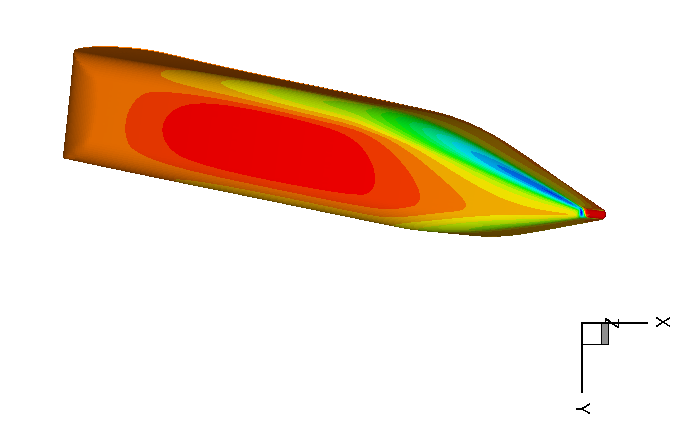
\includegraphics[height=0.15\textheight]{images/RANS_m6}\label{fig:ftf_snapshot}}\quad
  \subfigure[Flap Track Fairing DoF]
  {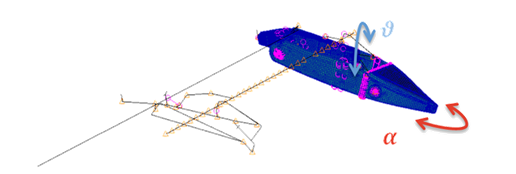
\includegraphics[height=0.15\textheight]{images/ftf_dof}\label{fig:ftf_dof}}\quad
      \caption{Details of the Flap track Fairing}
\end{figure*}


The FTF degree of freedom chosen for this analysis are $\theta$, the rotation around the longitudinal axis of the FTF, and $\alpha$ the rotation around the {\it spigot} axis, main connection between the track and the wing structure figure \ref{fig:ftf_dof}. The surface mesh of the CFD skin contains almost 36k nodes more precisely \(N_{nodes} = 36802\). We run the simulation for 9 different values of \(\alpha\) and 9 different values of \(\theta\), more precisely we have run the CFD-Rans computation for \(N_{parameter} = 9\times9 = 81\) number of times. In this particular case Reynolds Averaged  Navier-Stokes, {\it RANS}, equations are used with Spalart-Allmaras turbulence model to simulate the flow around the FTF. Figure \ref{fig:ftf_snapshot} shows one particular pressure snapshot. 

We use Leave One Out (LOO) Cross Validation method to quantify the performance of the two methodologies. $[\alpha, \theta]$ pairs are removed one by one from the database to create a new training set. The new training set is used to perform interpolation according to POD+I and distributed GP. Pressure snapshot is reconstructed for the missing $[\alpha, \theta]$ pairs. The methods are finally compared by evaluating the Root Mean Square Error (RMSE) and time of prediction values for each pair case. 

As described in Section \ref{sec:podi} we use all the available modes for pressure snapshot reconstruction. While performing distributed GP regression, we learn a GP model between \(p_{ij}\) and input vector \(X = [\Omega, \alpha, \theta]\). Effectively we are learning a GP model for \(N = 36802\times80 = 2.9\) million data-points. Since the input vector \(X\) is 5 dimensional, we propose to use Mat\'ern kernel for interpolating over the subsonic regime (subsection \ref{subsubsec:matern}).  

\begin{figure*}[!ht]
  \centering
  \subfigure[{Box plots of normalized RMSE for the two different model types. POD has a RMSE of \(0.48\pm0.27\) whereas distributed GP has a RMSE of \(0.37\pm0.1\). The mean distributed GP prediction is \(20\%\) better than POD. Outliers are extrapolation cases }]
  {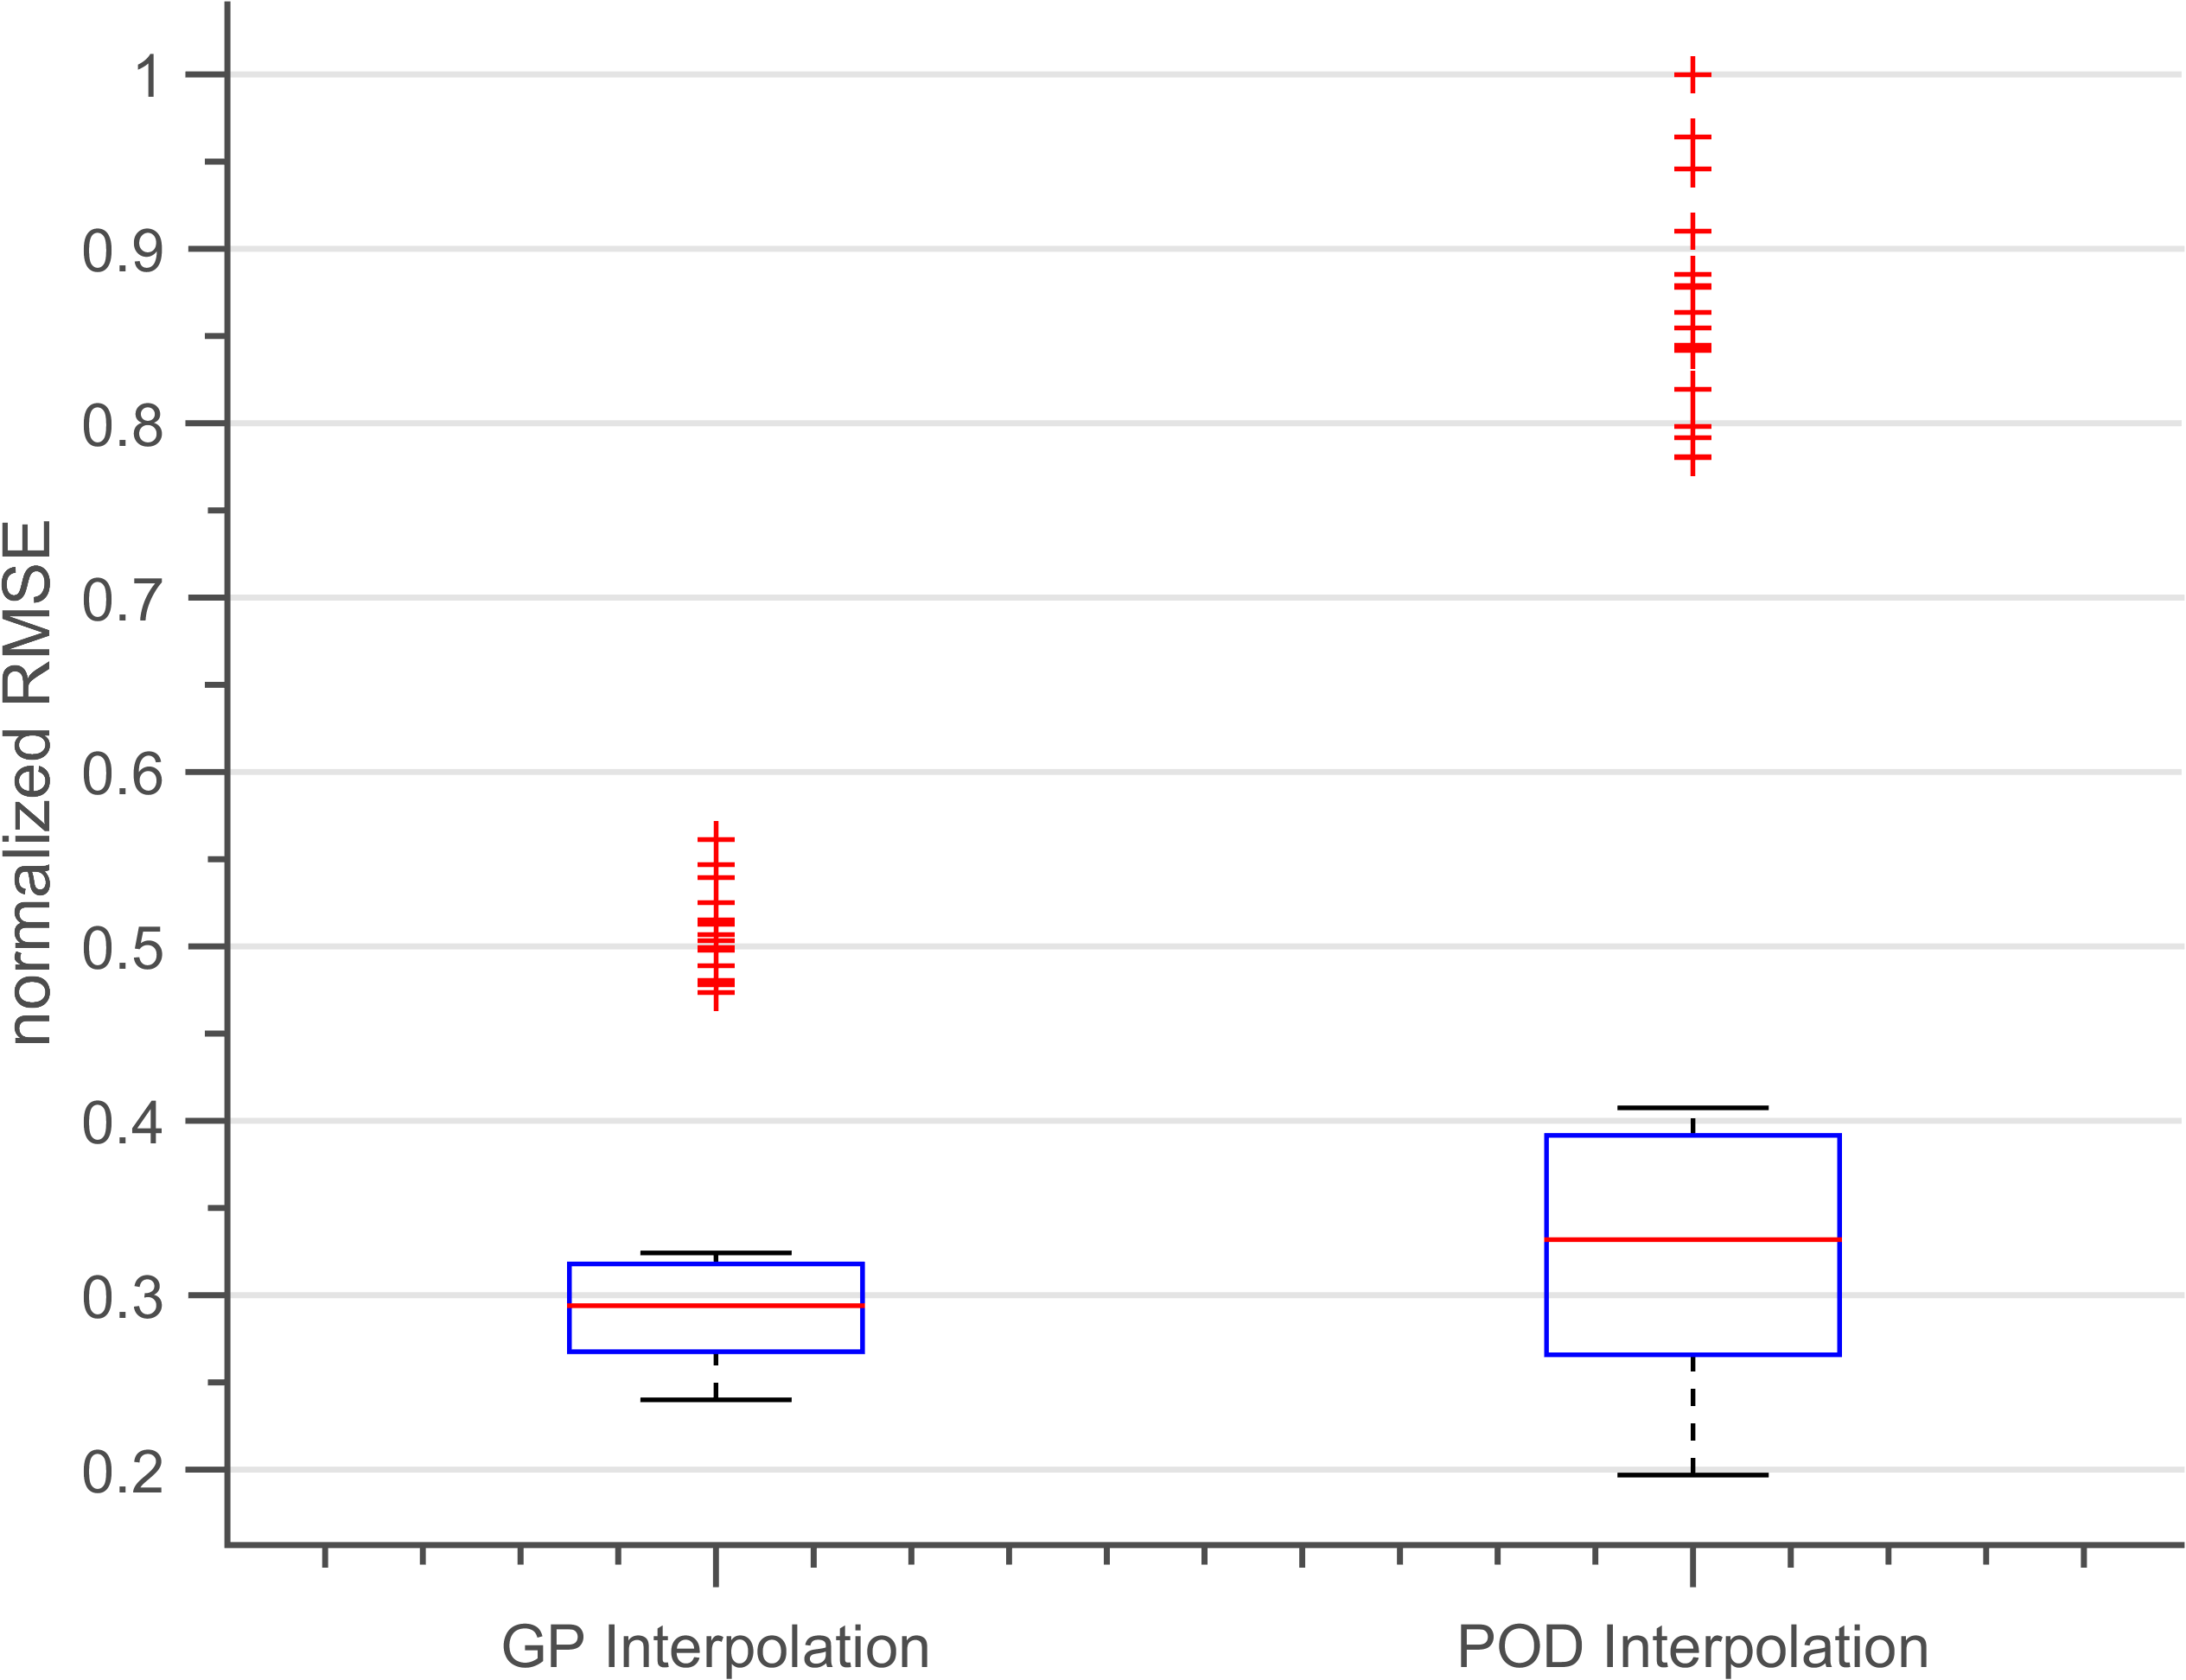
\includegraphics[width=0.45\textwidth]{images/rmse_AST}\label{subfig:RMSECFD}}\quad
    \subfigure[{Time taken to perform prediction for the two different model types. 
    POD takes \(2.35s\pm0.11s\) whereas distributed GP takes \(37.84s\pm4.35s\) to perform the interpolation. The average POD method is 19 times faster than distributed GP.}]
    {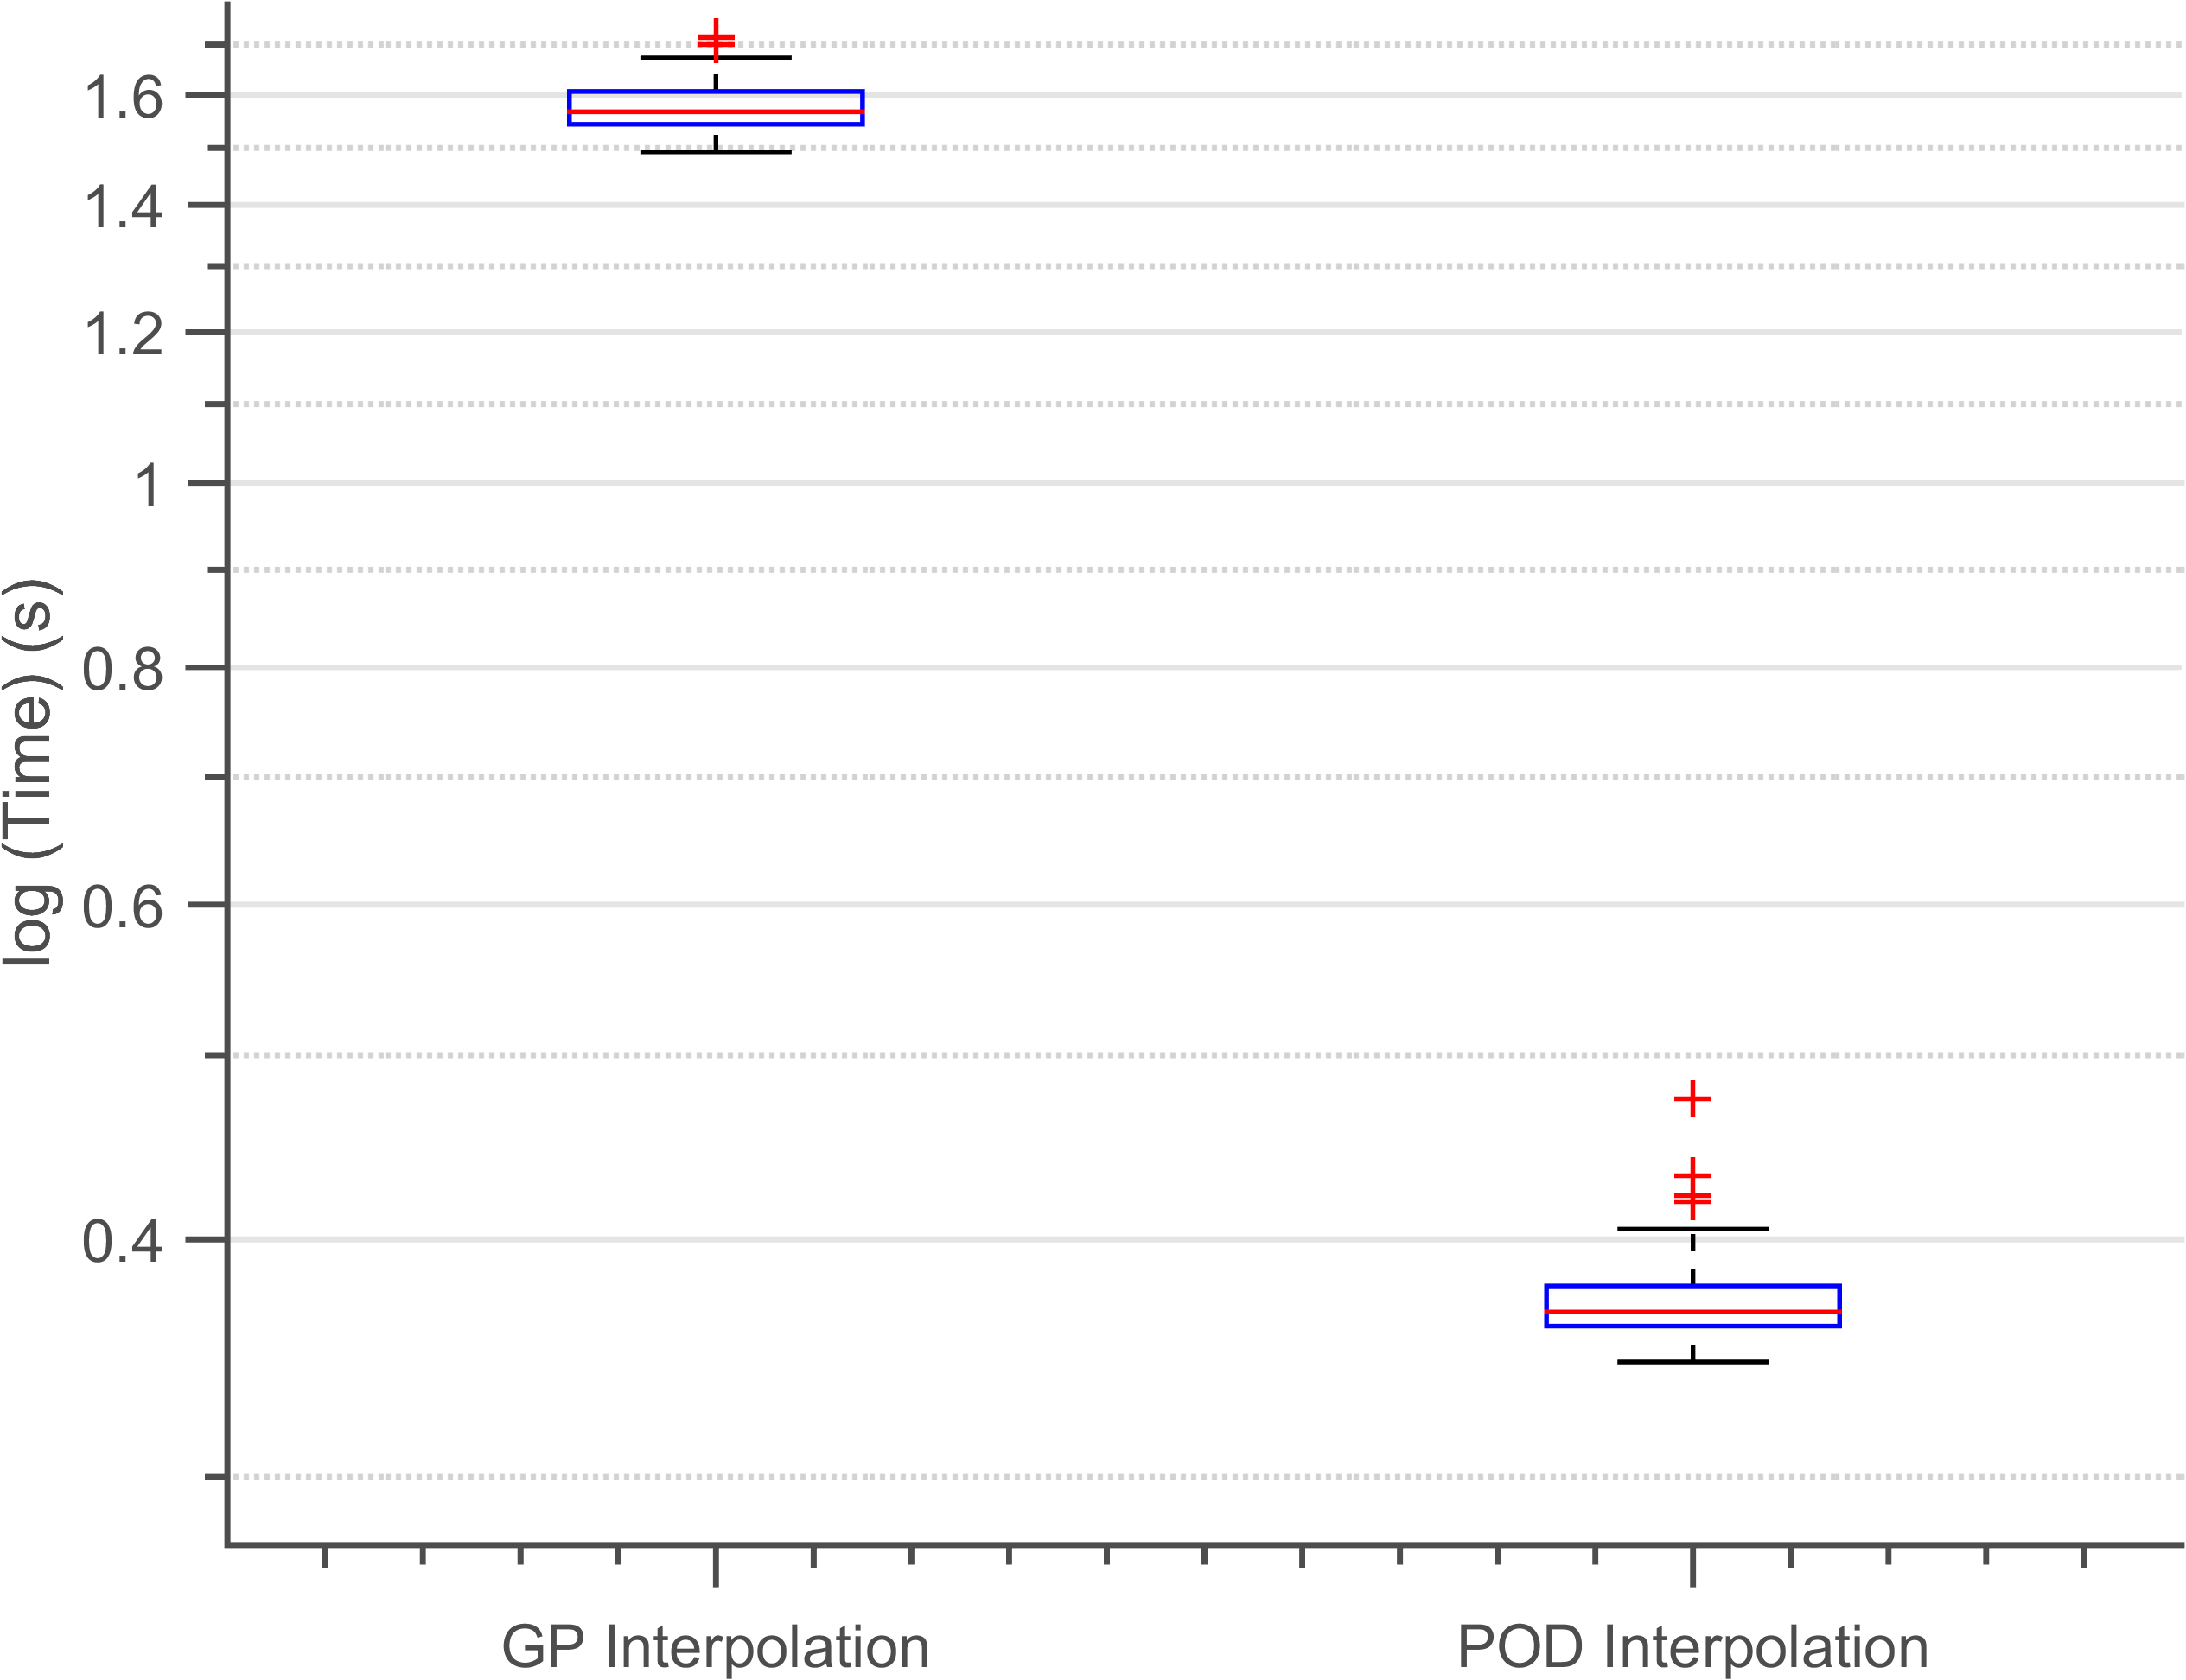
\includegraphics[width=0.45\textwidth]{images/time_AST}\label{subfig:timeCFD}}
  \caption{Results for elsA interpolation}
\end{figure*}

Figures \ref{subfig:RMSECFD} denote the RMSE estimates for different pairs. For RMSE distributed GP performs marginally better than POD. The outliers in the boxplots denote cases where the removed pairs are on the edges of database. Since the removed pairs are on the edges of database matrix, there are no CFD snapshots surrounding these pairs. Hence extrapolation is performed during the edge cases. POD has a RMSE of \(0.48\pm0.27\) whereas distributed GP has a RMSE of \(0.37\pm0.1\). The average distributed GP prediction is \(20\%\) better than POD. Figure \ref{subfig:timeCFD} shows the time taken to perform prediction for the two model types. POD takes \(2.35s\pm0.11s\) whereas distributed GP takes \(37.84s\pm4.35s\) to perform the interpolation. The POD method is the fastest sometimes performing 30 times faster than large scale GP. 

Although the GP technique can more efficiently capture non-linear behavior we see a relatively low improvement in performance for the amount of time invested. Deciding between the simple and time-tested POD method or costly and accurate distributed GP interpolation in the subsonic regime can be a tough task and mostly depends on the preferences of the final user.

\subsection{Interpolating in transonic regime}\label{subSec:resultsCRM}
We now proceed to compare the accuracy of the two methods in transonic regime on the Common Research Model (CRM)  proposed by NASA. Since the introduction of the model for the 4th Drag Prediction Workshop, the CRM has been become a very widely used test case for applied computational aerodynamics. Due to the widespread experience and availability of wind-tunnel test results for the configuration this is a natural case to benchmark interpolations. 

Due to the shape of an airfoil, airflow is accelerated on the upper surface of the wing. This causes shocks to appear on the upper surface of the wing in the transonic regime. Shocks are sudden changes (almost discontinuous) in the pressure and are important for estimating performance of the aircraft. Moreover an aircraft flies in the transonic regime for 80\% of its journey (cruise). Hence accurate prediction of location and strength of a shock is very important during design. Since POD is a linear subspace reduction method it has difficulty while reconstructing shock regime.

\begin{figure*}[!ht]
  \centering
  \subfigure[{Common research model. The four red lines are the four cuts at \(y/b = [0.105, 0.37, 0.5, 0.84]\). Here, \(y\) denotes the y-distance from aircraft axis and \(b\) denotes the span of one wing}.]
  {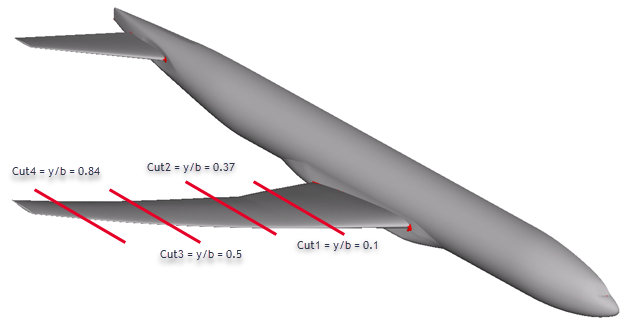
\includegraphics[width=0.45\textwidth]{images/crm_Wing_design}\label{subfig:crmWing}}\quad
    \subfigure[{Pressure snapshot on the Common Research model for \(\alpha = 2\) and \(Mach = 0.85\). We can observe double shock pattern appearing on the outer sections of the wing}]
    {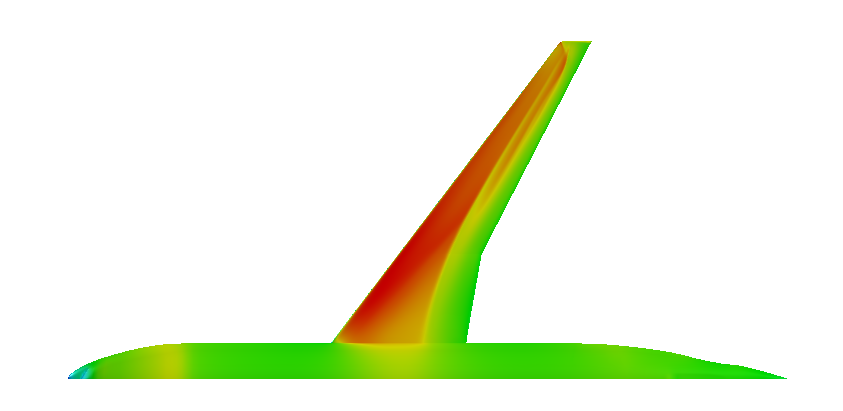
\includegraphics[width=0.45\textwidth]{images/surfM85A2}\label{subfig:crmSnapshot}}
  \caption{Common Research Model}
\end{figure*}

Again we use the elsA\textsuperscript{\textregistered} solver to perform simulations on the design. We use the \(\kappa - \omega\) SST turbulence model to perform predictions since it has good performance in the fuselage wing interaction regions \cite{menter2003ten, vassberg2014summary}. The CFD was run for a combination of 21 values of \(\alpha \in [1: 0.1: 3]\) and 5 values of \(Mach \in [0.84: 0.005: 0.86]\), hence \(N_{parameter} = 21\times5 = 105\). Figure, \ref{subfig:crmSnapshot} shows one of the pressure snapshots for \(\alpha = 2\) and \(Mach = 0.85\). We then cut the wing at four distinct locations \(y/b = [0.105, 0.37, 0.5, 0.84]\) figure \ref{subfig:crmWing} to clearly observe different types of aerodynamic behavior. Here, \(y\) denotes the y-distance from aircraft axis and \(b\) denotes the span of one wing. 

As detailed in the earlier section we again use LOO-CV for comparing the performance of the two methods. The POD+I method has been run as described in Section \ref{sec:podi}. The distributed GP has been run as described in the earlier section only this time we use Neural Network kernel for the spatial dimension. The neural network kernel lets us encode information of discontinuity (as expected from a shock) in our family of functions as detailed in subsection \ref{subsubsec:nnkernel}. 

\begin{figure*}[!ht]
  \centering
  \subfigure[{Normalized RMSE for the two different model types. POD has a RMSE of \(0.32\pm0.23\) whereas distributed GP has a RMSE of \(0.02\pm0.01\). The average distributed GP prediction is 16 times better than POD in transonic regime. The outliers in the boxplots denote cases where the removed pairs are on the edges of database. Since the removed pairs are on the edges of database matrix, there are no CFD snapshots surrounding these pairs. Hence extrapolation is performed during the edge cases.}]
  {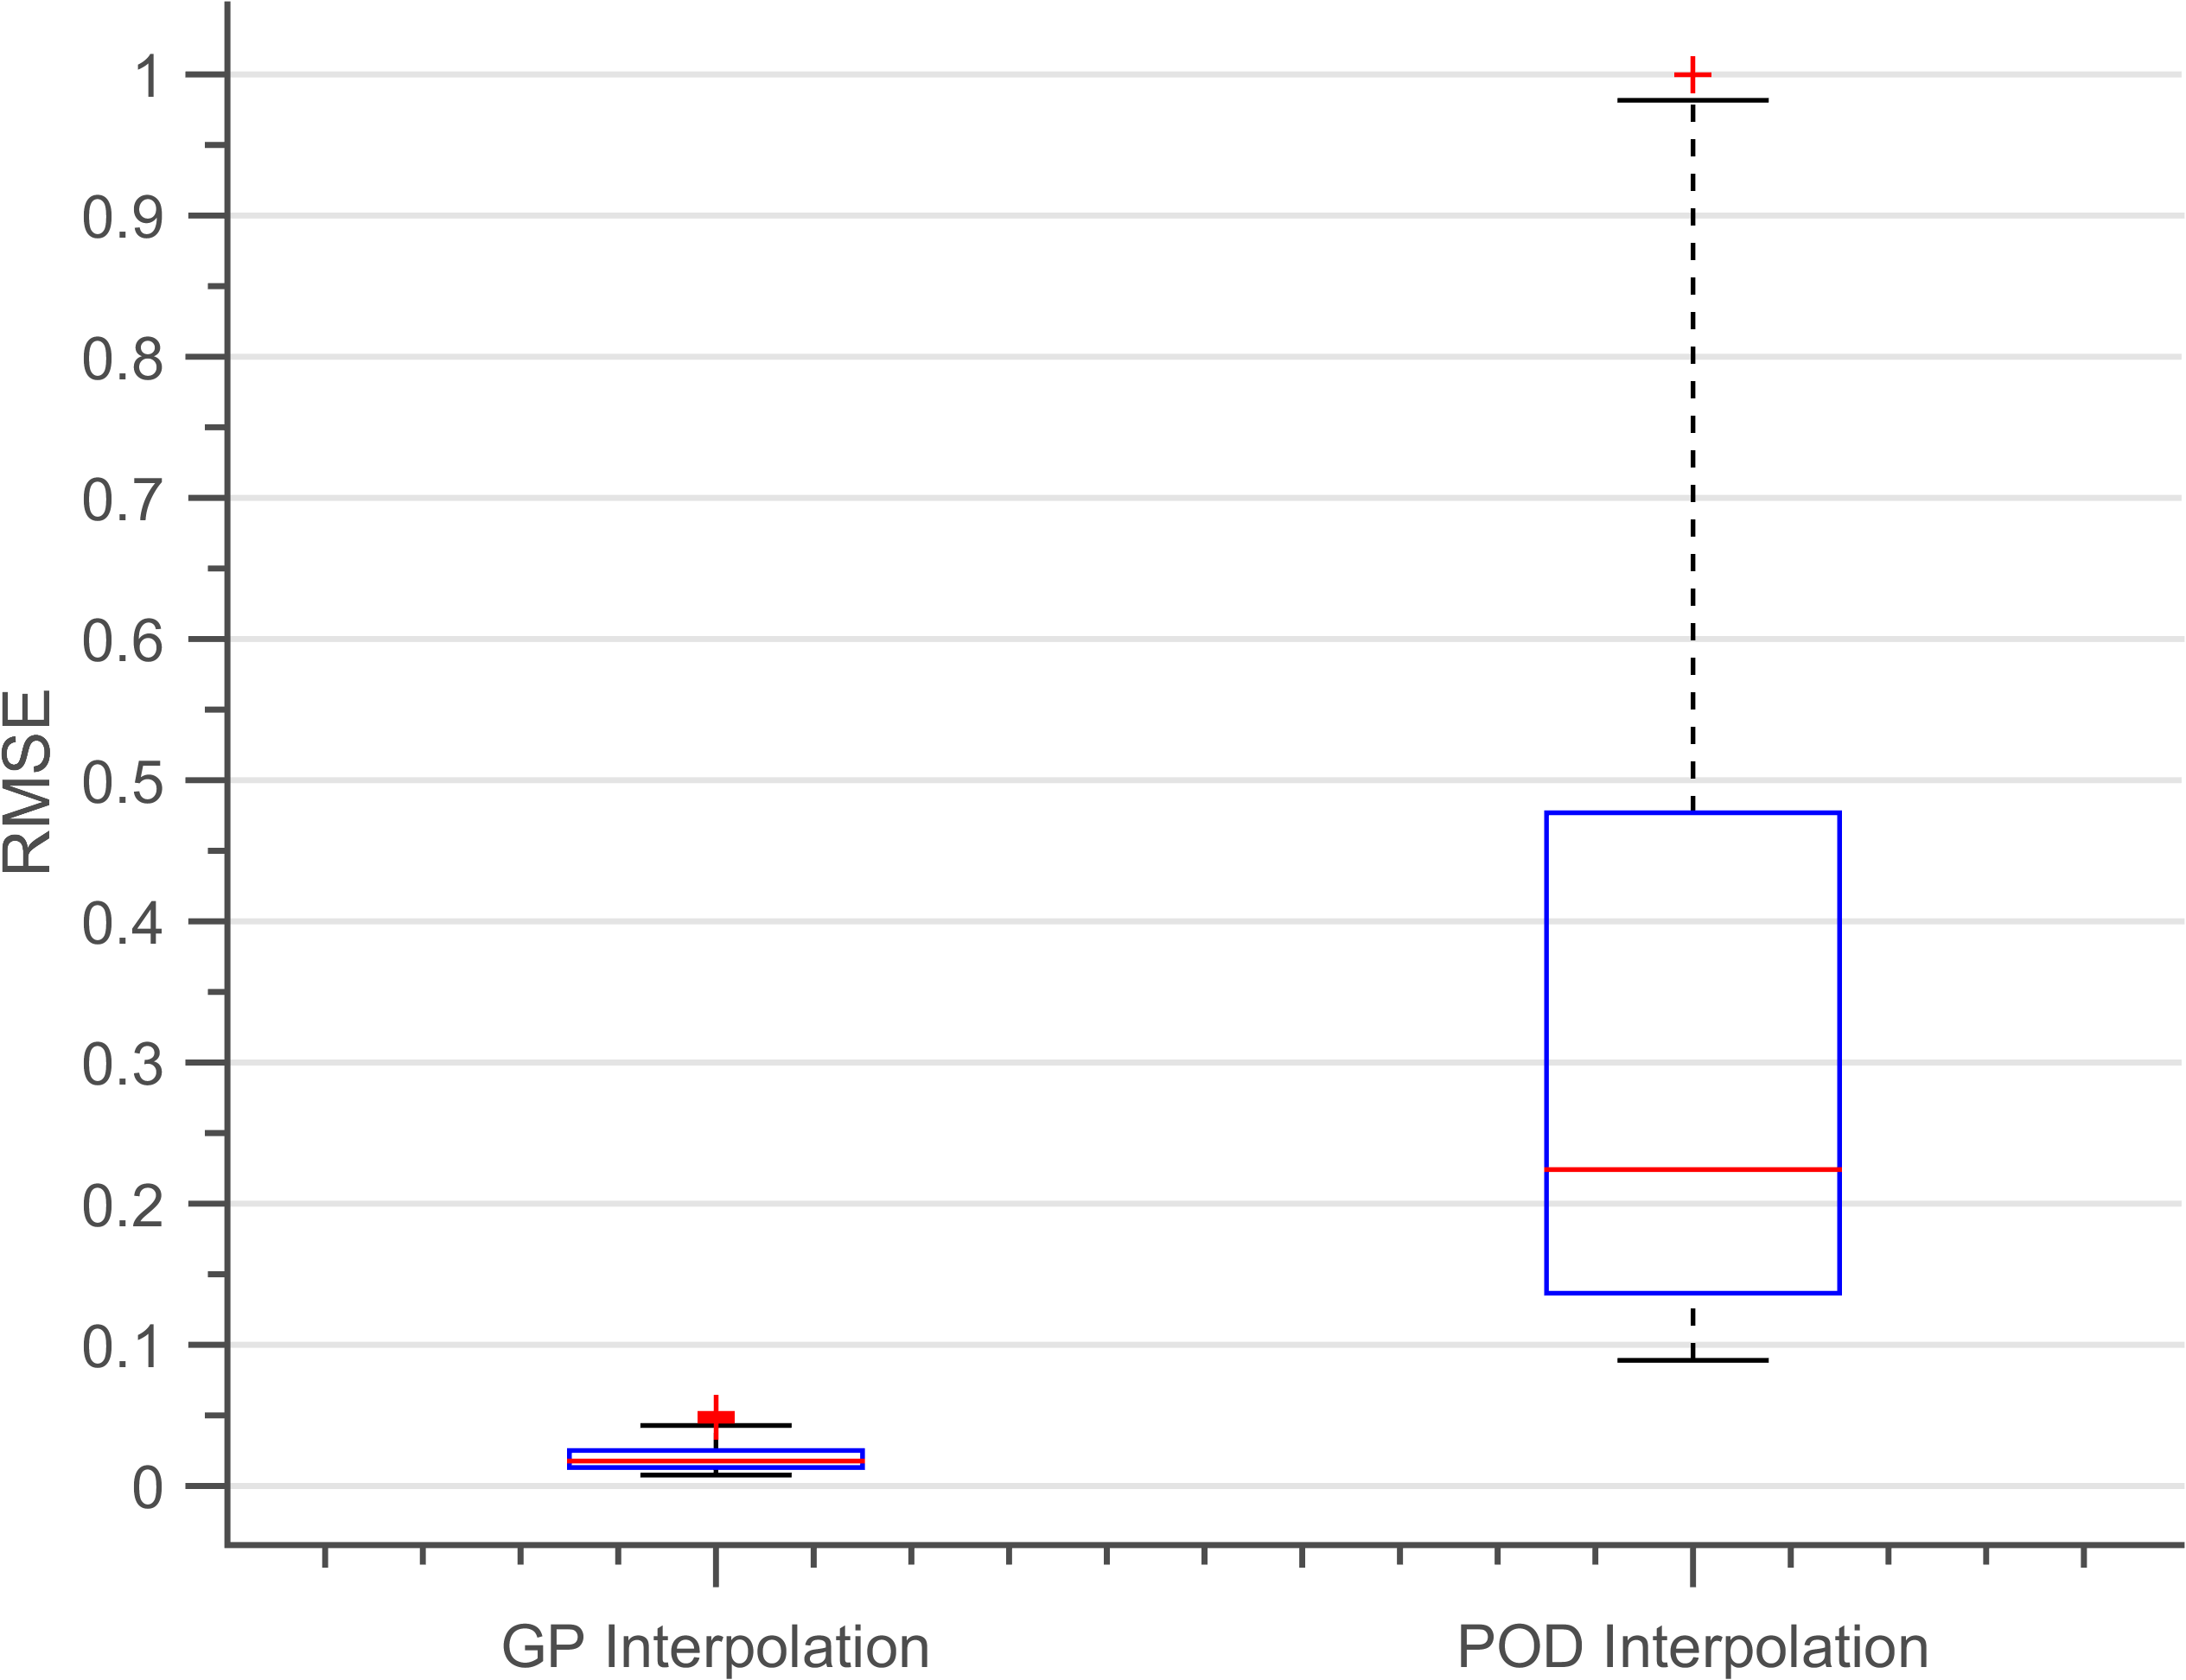
\includegraphics[width=0.45\textwidth]{images/rmseCRM_box}\label{subfig:RMSECRM}}\quad
    \subfigure[{Time taken to perform prediction for the two different model types. The x axis denotes indices of removed pairs. POD takes \(0.5s\pm0.03s\) whereas distributed GP takes \(40.6s\pm2.3s\) to perform the interpolation. The average POD method is 80 times faster than distributed GP. Here we are interpolating the pressure on the whole wing.}]
    {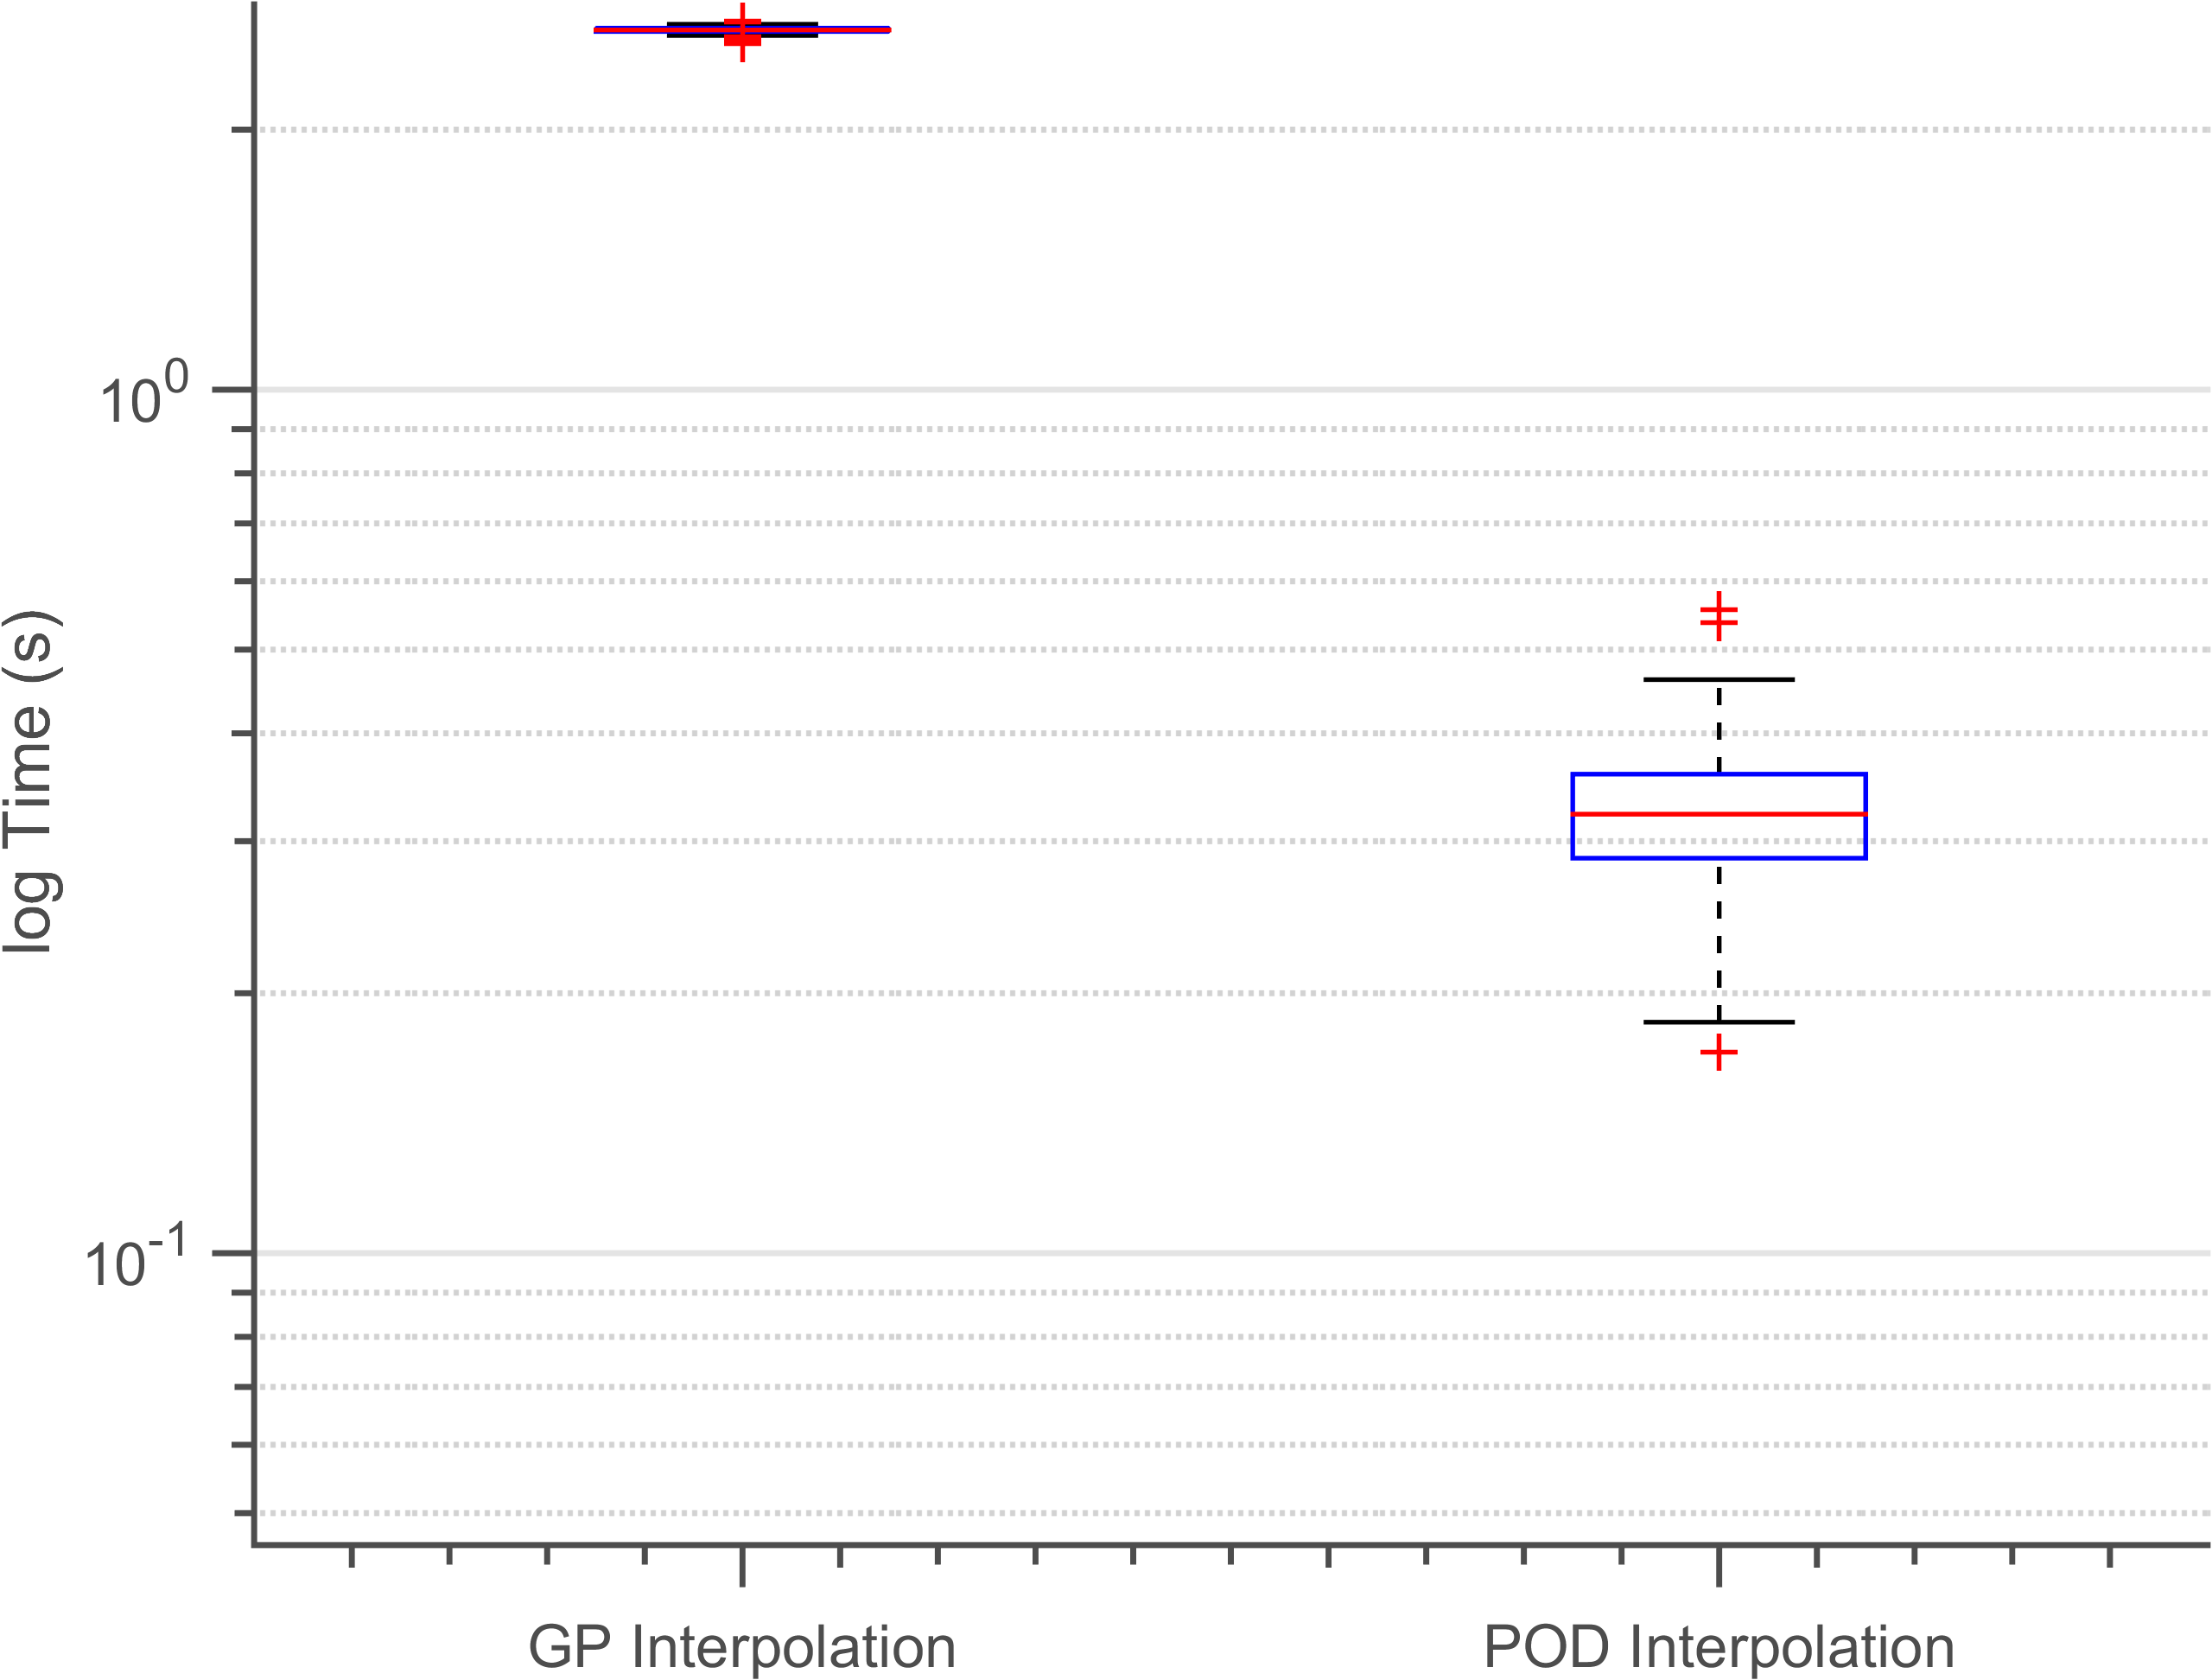
\includegraphics[width=0.45\textwidth]{images/timeCRM_box}\label{subfig:timeCRM}}
  \caption{Results for CRM interpolation}
\end{figure*}

The above figures \ref{subfig:RMSECRM} denote the RMSE estimates for different pairs. POD has a RMSE of \(0.32\pm0.23\) whereas distributed GP has a RMSE of \(0.02\pm0.01\). The average distributed GP prediction is 16 times better than POD in transonic regime. The outliers in the boxplots denote cases where the removed pairs are on the edges of database. Since the removed pairs are on the edges of database matrix, there are no CFD snapshots surrounding these pairs. Hence extrapolation is performed during the edge cases. Figure \ref{subfig:timeCRM} shows the time taken to perform prediction for the three different model types. The x axis denotes indices of removed pairs. POD takes \(0.5s\pm0.03s\) whereas distributed GP takes \(40.6s\pm2.3s\) to perform the interpolation. In transonic regime GP has a significantly better error performance and becomes the obvious choice for interpolation.

\begin{figure*}[!ht]
  \centering
  \subfigure[{Comparison between POD method and distributed GP for interpolation. The X-axis denotes chord dimension, only showing chord-section near shock for clarity. The Y-axis denotes the coefficient of pressure. Reconstruction is performed on the pressure snapshot at \(\alpha = 2\) and \(Mach = 0.85\) for the \(y/b = 0.105\)}. We can observe that the intensity of shock has been smoothed out by POD method]
  {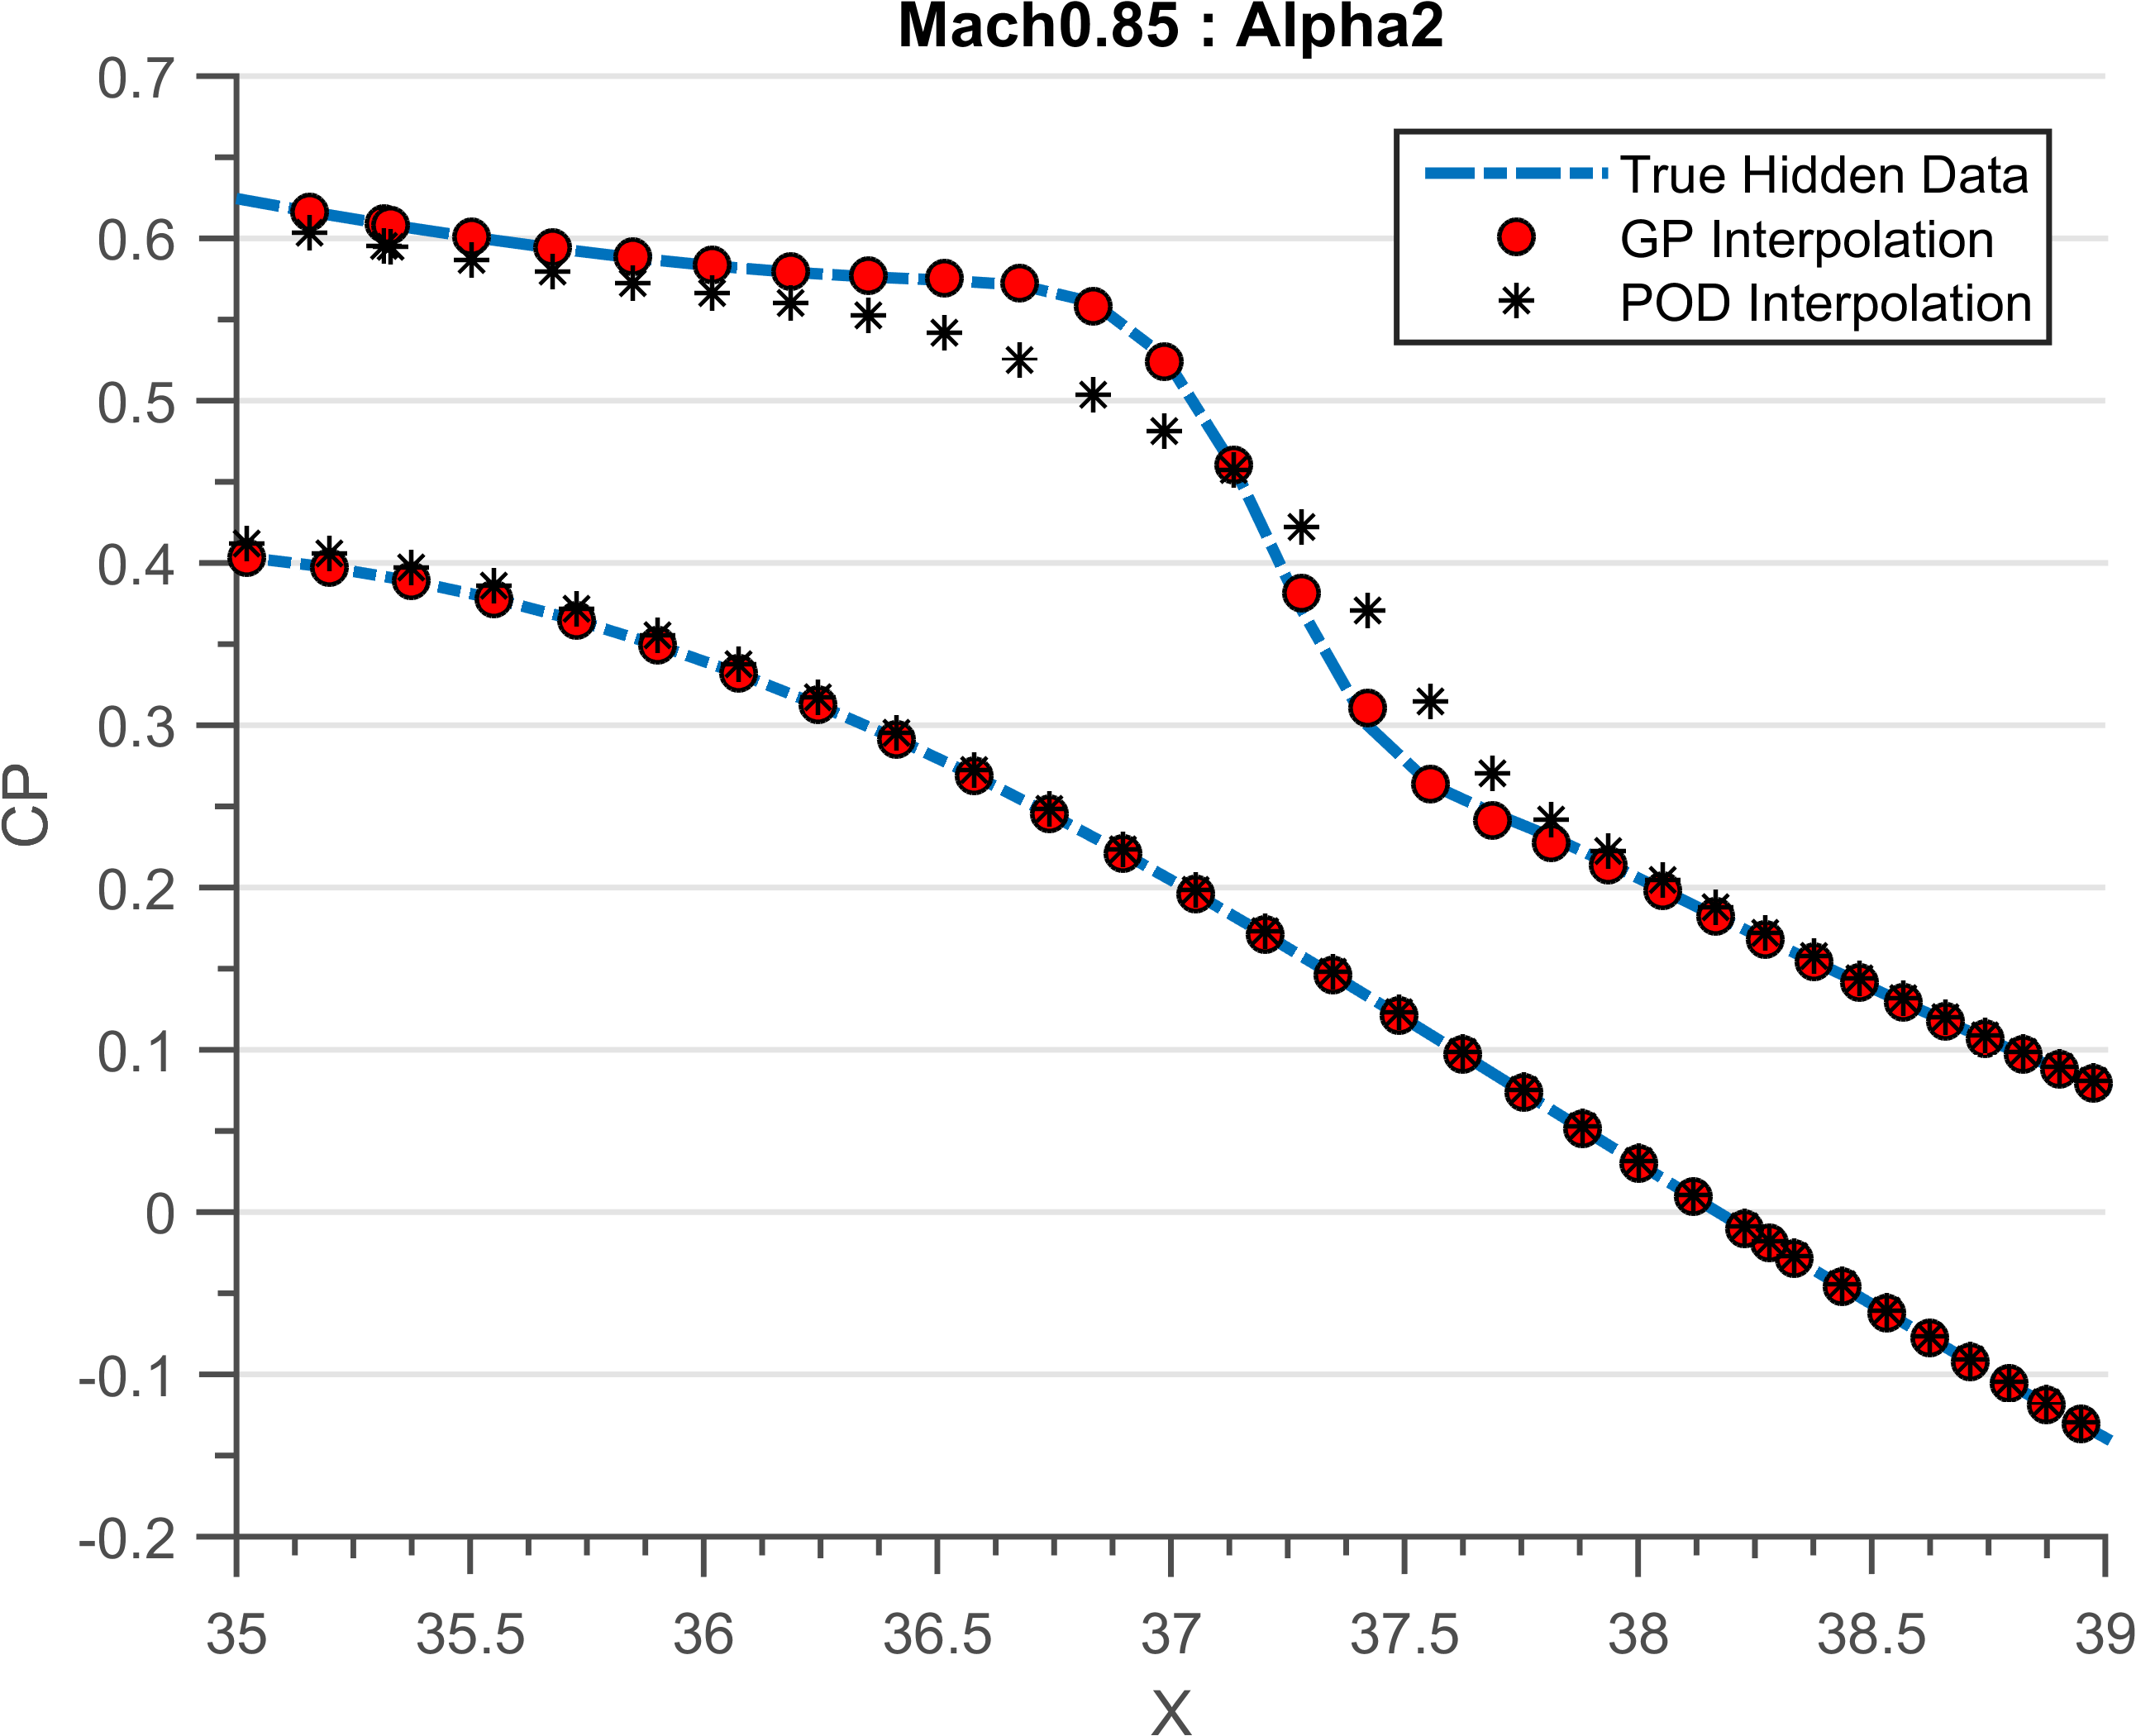
\includegraphics[width=0.45\textwidth]{images/CRM-clean-testSnapshots_M850A20}\label{subfig:interpComparisonCRM}}\quad
    \subfigure[{Comparison between POD method and distributed GP for extrapolation. The X-axis denotes chord dimension, only showing chord-section near shock for clarity. The Y-axis denotes the coefficient of pressure. Reconstruction is performed on the pressure snapshot at \(\alpha = 2\) and \(Mach = 0.84\) for the \(y/b = 0.105\). We can observe that POD introduces errors both for the intensity of shock and location of shock for this case}]
    {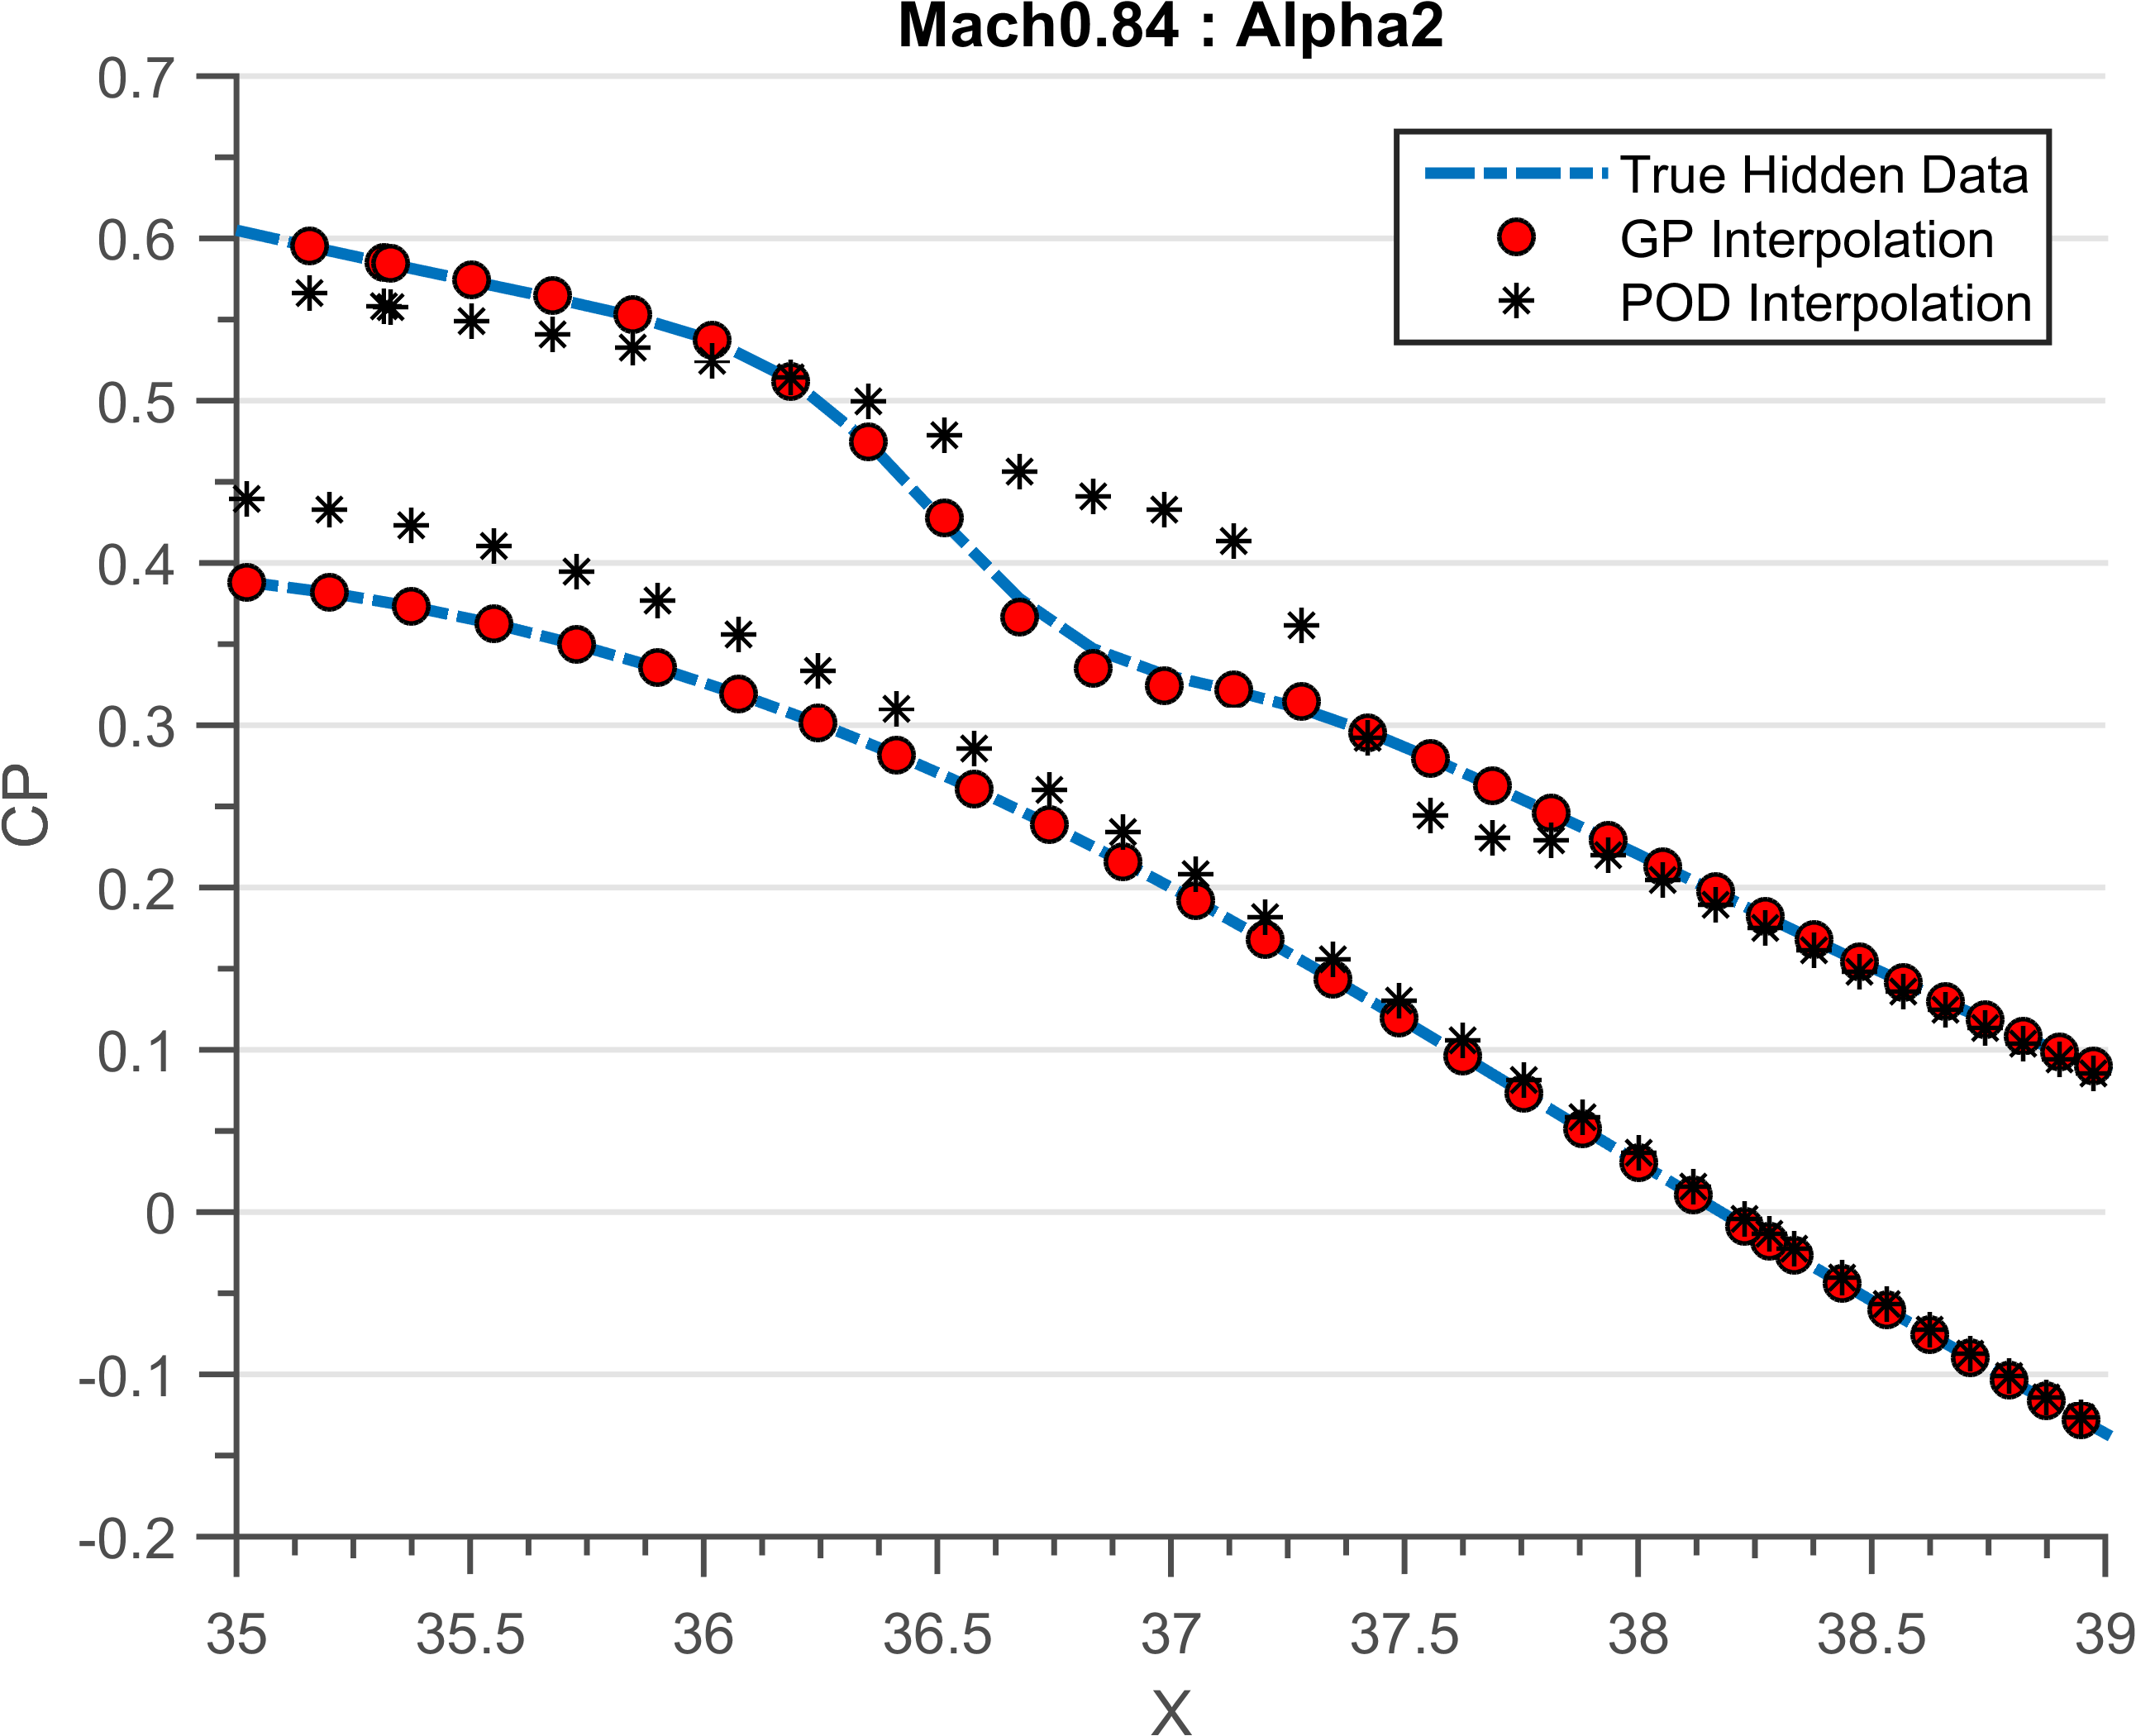
\includegraphics[width=0.45\textwidth]{images/CRM-clean-testSnapshots_M840A20}\label{subfig:exterpComparisonCRM}}
  \caption{Comparison of pressure interpolations for first cut \(y/b = 0.105\). Here we compare the accuracy of prediction for interpolation and extrapolation cases.}
\end{figure*}

Figure \ref{subfig:interpComparisonCRM} shows the comparison between POD method and distributed GP for interpolation. Reconstruction is performed on the pressure snapshot at \(\alpha = 2\) and \(Mach = 0.85\) for the \(y/b = 0.105\). We can observe that the shape of shock has been smoothed out by POD method. Figure \ref{subfig:exterpComparisonCRM} shows comparison between POD method and distributed GP for extrapolation. Reconstruction is performed on the hidden pressure snapshot of \(\alpha = 2\) and \(Mach = 0.84\) which is an edge case. We can observe that POD introduces errors both for the intensity of shock and location of shock for the extrapolation case, this explains the high amount of error in figure \ref{subfig:RMSECRM}.  

\subsubsection{Comparison across cuts}
We next study the accuracy of distributed GP for different airfoils on the wing. Using the methodology described earlier we build a distributed GP model for each airfoil and measure the accuracy of interpolation performed for each cut using the LOO-CV methodology. 

\begin{figure*}[!ht]
  \centering
  \subfigure[{Normalized RMSE for different airfoils based on distributed GP. The mean RMSE of different cuts from \(y/b = [0.105, 0.37, 0.5, 0.84]\) is \([0.053, 0.17, 0.31, 0.40]\) respectively. The accuracy of interpolation deteriorates as we go farther away from the fuselage. This is due to appearance of double shock on the outer section of wing.}]
  {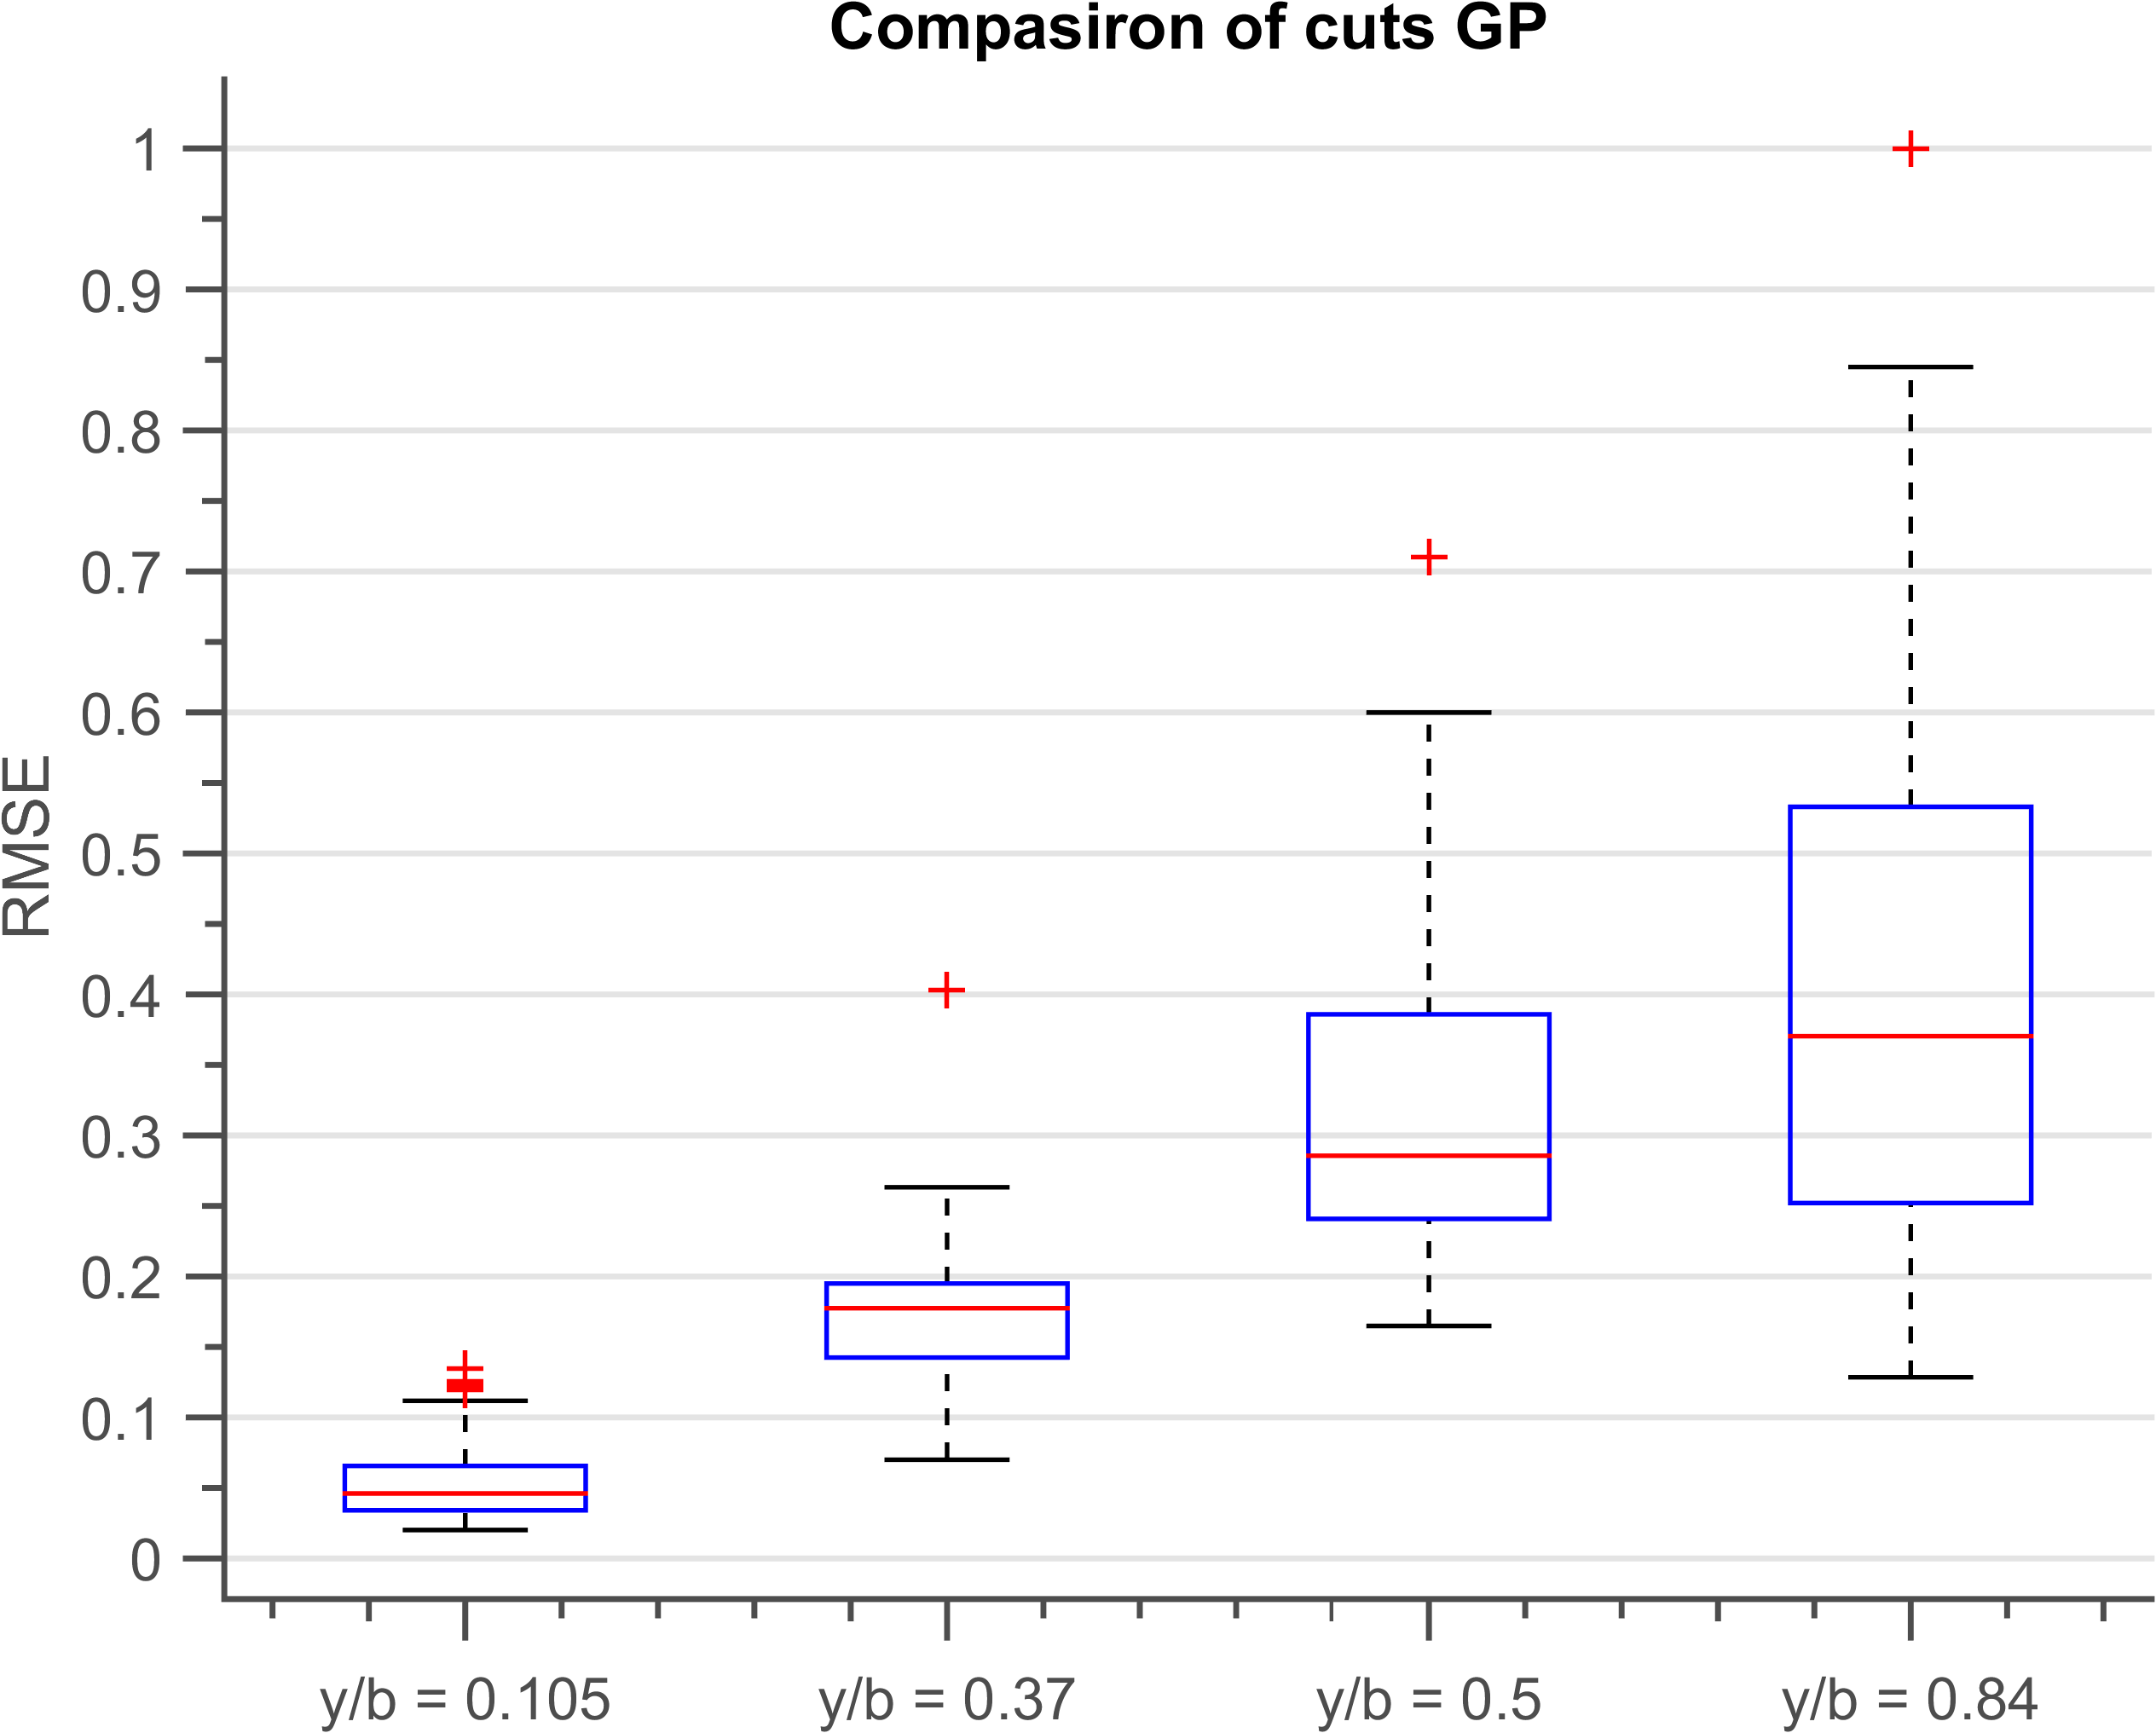
\includegraphics[width=0.45\textwidth]{images/compasironOfCutsGPCRM_box}\label{subfig:compasironOfCutsGPCRM}}\quad
    \subfigure[{Comparison between POD method and distributed GP for interpolation. The X-axis denotes chord dimension, only showing chord-section near shock for clarity. The Y-axis denotes the coefficient of pressure. Reconstruction is performed on the pressure snapshot at \(\alpha = 2\) and \(Mach = 0.85\) for the location  \(y/b = 0.84\)}. While POD smooths out the double shock pattern distributed GP also lacks the accuracy observed in figure \ref{subfig:interpComparisonCRM}.]
    {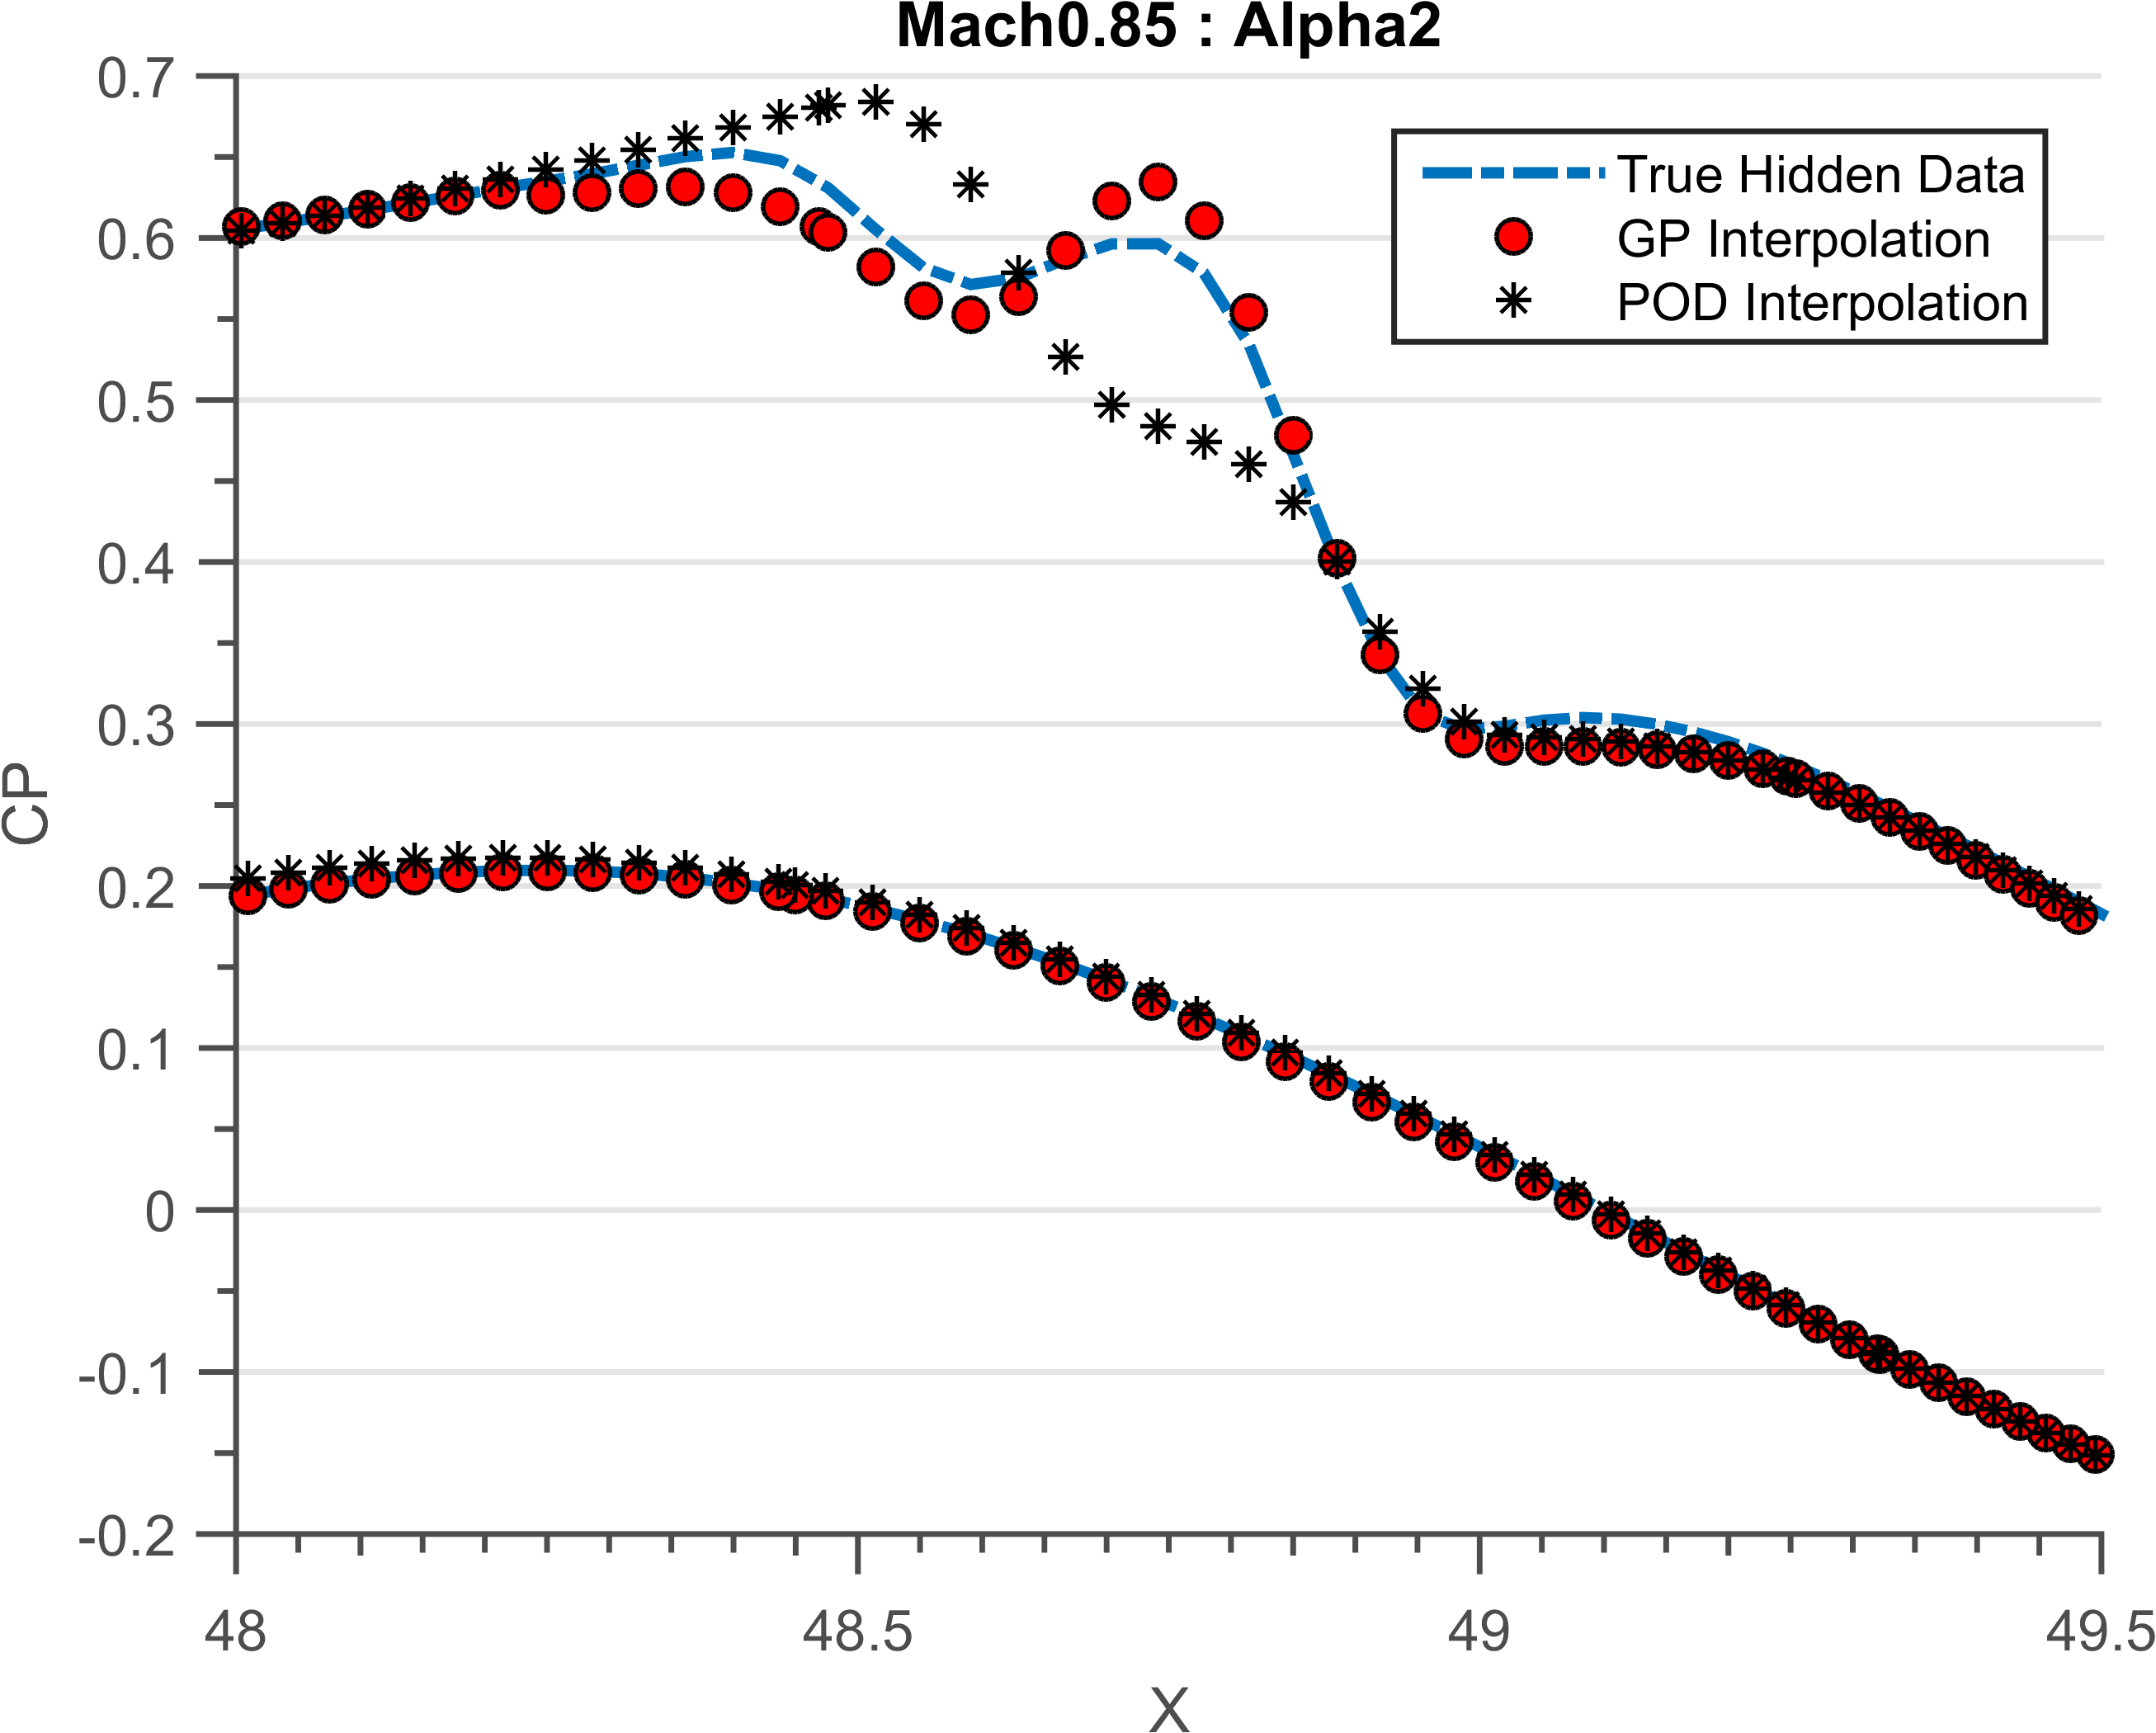
\includegraphics[width=0.45\textwidth]{images/CRM-clean-testSnapshots_M850A20_cut4}\label{subfig:interpCut4}}
  \caption{Performance of distributed GP across cuts}
\end{figure*}

Figure \ref{subfig:compasironOfCutsGPCRM} shows the RMSE performance across cuts. The performance of interpolation deteriorates as we go further away from the fuselage. This is primarily because as we go further away from the fuselage double shocks start appearing on the airfoil as observable from figure \ref{subfig:crmSnapshot}. Figure \ref{subfig:interpCut4} shows interpolation performed by the POD method and distributed GP methods at \(\alpha = 2\) and \(Mach = 0.85\). While, POD smooths out the double shock pattern distributed GP also lacks the accuracy observed in figure \ref{subfig:interpComparisonCRM}. 

\begin{figure*}[!ht]
  \centering
  \subfigure[{Interpolation performed at constant \(Mach = 0.845\) and \(\alpha = [1, 3]\) for the location \(y/b = 0.105\). The color coding denotes coefficient of pressure for upper side of airfoil, The x-axis denotes chord-wise location and y-axis denotes \(\alpha\). White lines denote presence of a pressure snapshot due to CFD run, everything in between is interpolation. Dashed black lines denote constant pressure contours color between two contours has been smoothed for clarity. We observe a strong shock near \(\alpha = 3\) which slowly gets converted to a weak shock near \(\alpha = 1\).}]
  {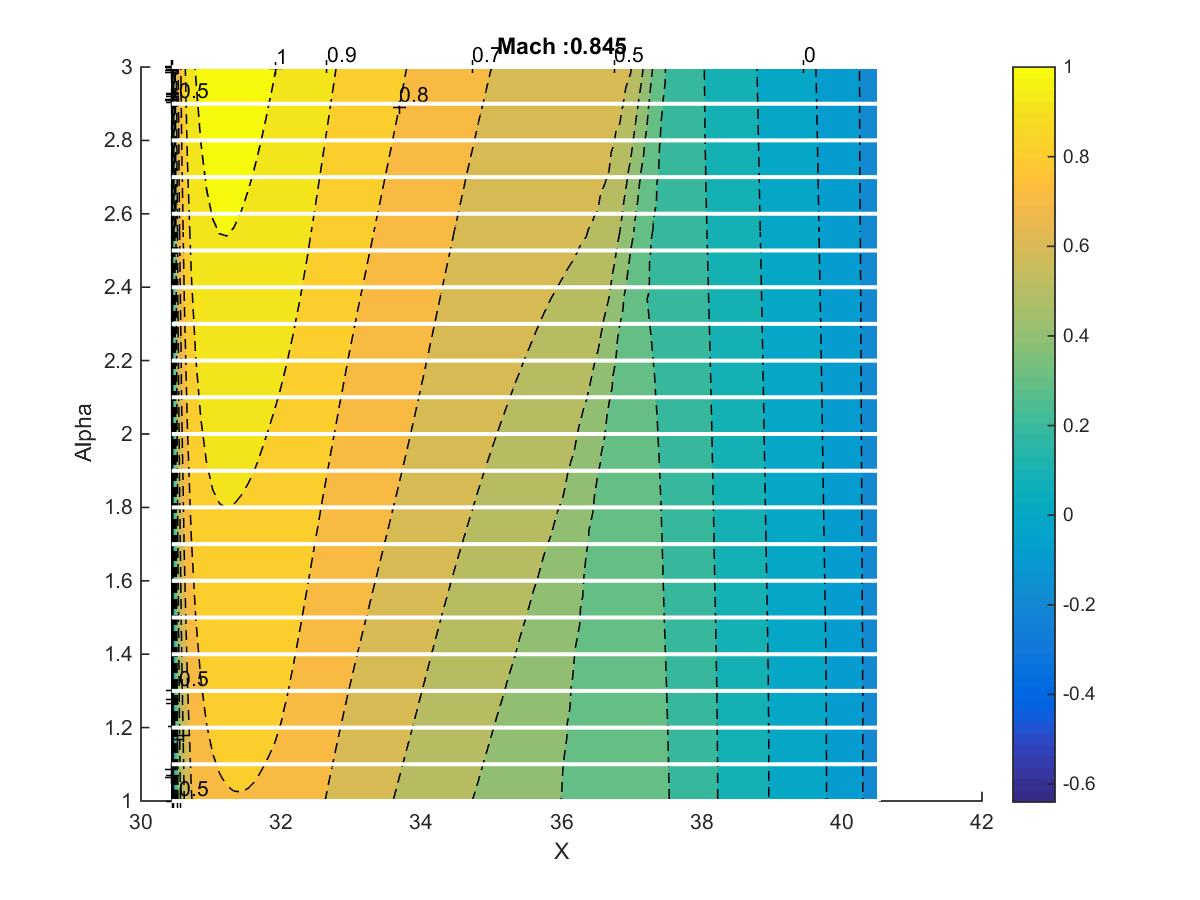
\includegraphics[width=0.45\textwidth]{images/CRM-clean-testSnapshots_cut1_MachSweepContF845}\label{subfig:alphaSweepCut1}}\quad
    \subfigure[{Interpolation performed at constant \(Mach = 0.845\) and \(\alpha = [1, 3]\) for the location \(y/b = 0.84\). The color coding denotes coefficient of pressure for upper half of airfoil, The x-axis denotes chord-wise location and y-axis denotes \(\alpha\). White lines denote presence of a pressure snapshot due to CFD run, everything in between is interpolation. Dashed black lines denote constant pressure contours color between two contours has been smoothed for clarity. We observe a single shock near \(\alpha = 3\) which slowly gets converted to a double shock pattern.}]
    {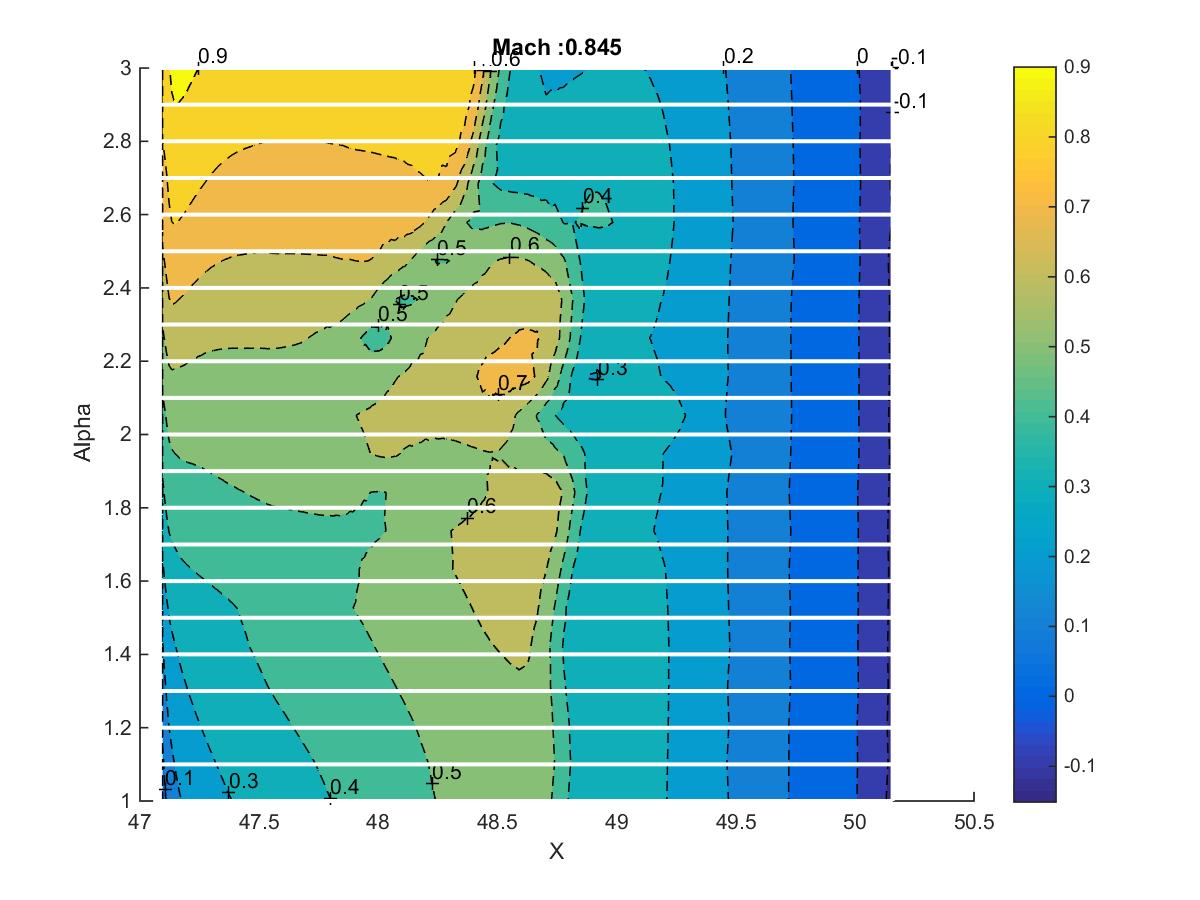
\includegraphics[width=0.45\textwidth]{images/CRM-clean-testSnapshots_cut4_MachSweepContF845}\label{subfig:alphaSweepCut4}}
  \caption{Pressure reconstructions for constant \(Mach = 0.845\) and sweeping \(\alpha \in [1, 3]\)}
\end{figure*}

Figures \ref{subfig:alphaSweepCut1} and \ref{subfig:alphaSweepCut4} show the evaluation of pressures upon varying \(\alpha \in [1, 3]\) at locations \(y/b = 0.105\) and \(y/b = 0.84\) respectively. The color coding denotes coefficient of pressure for upper side of airfoil, The x-axis denotes chord-wise location and y-axis denotes \(\alpha\). White lines denote presence of a pressure snapshot due to CFD run, everything in between is interpolation. Dashed black lines denote constant pressure contours Color between two contours has been smoothed for clarity. For figure \ref{subfig:alphaSweepCut1} we observe a strong shock near \(\alpha = 3\) which slowly gets converted to a weak shock near \(\alpha = 1\). The presence of a single shock is also the reason why distributed GP performs better at this cut location. For figure \ref{subfig:alphaSweepCut4} we observe a single shock near \(\alpha = 3\) which slowly gets converted to a double shock pattern. The zone of from single to double shock is a very interesting point for performance, since the wing drag is minimum during this transition phase. Distributed GP starts performing badly near the transition phases, this can be observed by the small pools of \(C_{P} = 0.5\) at the transition phase from single to double shock. 


\subsection{Discussion}\label{subsec:ExpressingStructureKernelConclusion}
The above section shows a small sneak peek into the vast variety of kernel functions available in research papers. Due to the ability to create new kernels every problem statement comes up with an optimal structure which encodes the basic assumptions. Unfortunately finding the correct kernel is still a black art. 
 
As mentioned earlier the core aim of machine learning was to identify patterns and extrapolate on data automatically. There are two main approaches in pattern discovery; one which defines a language of kernels and iteratively adds basic kernels to come up with an explanation to the pattern in the data \cite{lloyd2014automatic}. The second is based on increasing the hypothesis space by defining a process over all stationary kernels \cite{wilson2012process}. Which approach will be retained in the long term is tough to say but research in automatic pattern detection is a highly active subject. 

It is also in the interest of this PhD to be able to extrapolate till limit-loads. Constructing a detailed kernel which can replace the parametric theoretical model is highly time-consuming. We wish to use the already constructed theoretical model as a prior into our model. How to use a parametric model for extrapolation will be discussed in the next section.

